\documentclass[10pt, a4paper]{report}

%%%%%%%%%%%%%%%%%%%%%%%%%%%%%%%%%%%%%%%%%
% Wenneker Article
% Structure Specification File
% Version 1.0 (28/2/17)
%
% This file originates from:
% http://www.LaTeXTemplates.com
%
% Authors:
% Frits Wenneker
% Vel (vel@LaTeXTemplates.com)
%
% License:
% CC BY-NC-SA 3.0 (http://creativecommons.org/licenses/by-nc-sa/3.0/)
%
% Adapted for COMS30007 by Carl Henrik Ek
% And then adapted for his Thesis by Leo Poulson
%
%%%%%%%%%%%%%%%%%%%%%%%%%%%%%%%%%%%%%%%%%

%----------------------------------------------------------------------------------------
%	PACKAGES AND OTHER DOCUMENT CONFIGURATIONS
%----------------------------------------------------------------------------------------

\usepackage[english]{babel} % English language hyphenation

\usepackage{microtype} % Better typography

\usepackage{amsthm} % Math packages for equations
\usepackage{amsmath}
\usepackage{amssymb}
\usepackage{mathtools}
\usepackage{bm}
\usepackage{xfrac}
\usepackage{resizegather}
\usepackage[]{algorithmicx}

\usepackage{minted}

\usepackage[weather]{ifsym}

\usepackage{wrapfig}


\usepackage[svgnames]{xcolor} % Enabling colors by their 'svgnames'

\usepackage[hang, small, labelfont=bf, up, textfont=it]{caption} % Custom captions under/above tables and figures

\usepackage{booktabs} % Horizontal rules in tables

\usepackage{lastpage} % Used to determine the number of pages in the document (for "Page X of Total")

\usepackage{graphicx} % Required for adding images

\usepackage{subcaption} % Add subfigures
\usepackage{enumitem} % Required for customising lists
\setlist{noitemsep} % Remove spacing between bullet/numbered list elements

\usepackage{sectsty} % Enables custom section titles
\allsectionsfont{\usefont{OT1}{phv}{b}{n}} % Change the font of all section commands (Helvetica)

\usepackage{tikz}

\usetikzlibrary{shapes.multipart} % Enables multi-line tikz nodes 
\usetikzlibrary{shapes.misc} % lets us use funny shapes
\usetikzlibrary{arrows,shapes,snakes,automata,backgrounds,petri}
\usetikzlibrary{positioning}

\usetikzlibrary{decorations.pathreplacing}

\usepackage{pgfplots}
\pgfplotsset{compat=1.9}
\usepgfplotslibrary{external}
%----------------------------------------------------------------------------------------
%	MARGINS AND SPACING
%----------------------------------------------------------------------------------------

\usepackage{geometry} % Required for adjusting page dimensions

\geometry{
	top=2cm, % Top margin
	bottom=2cm, % Bottom margin
	left=2cm, % Left margin
	right=2cm, % Right margin
	includehead, % Include space for a header
	includefoot, % Include space for a footer
	%showframe, % Uncomment to show how the type block is set on the page
}

\setlength{\columnsep}{7mm} % Column separation width

% --------------------------------------------------------
%   NEW COMMANDS
% --------------------------------------------------------

\newcommand{\mc}[1]{\mathcal{#1}}
\newcommand{\tmc}[1]{$\mathcal{#1}$}
\newcommand{\wh}[1]{\widehat{#1}}
\newcommand{\m}{\tmc{M}}
\newcommand{\e}{\tmc{E}}
\newcommand{\mm}{\mc{M}}
\newcommand{\me}{\mc{E}}
\newcommand{\rsarrow}{\rightsquigarrow}

\newcommand{\pre}{\textsf{pre}}
\newcommand{\post}{\textsf{post}}
\newcommand{\tpre}{$\pre$ }
\newcommand{\tpost}{$\post$ }

\newcommand{\mestar}{$\mathcal{ME^\ast}$ }

\newcommand{\secref}[1]{Section \ref{#1}}
\newcommand{\figref}[1]{Figure \ref{#1}}

\newcommand{\mih}[1]{\mintinline{haskell}{#1}}

% --------------------------------------------------------
%   NEW ENVIRONMENTS
% --------------------------------------------------------

\newenvironment{centermath}
 {\begin{center}$\displaystyle}
 {$\end{center}}

%----------------------------------------------------------------------------------------
%	FONTS
%----------------------------------------------------------------------------------------

\usepackage[T1]{fontenc} % Output font encoding for international characters
\usepackage[utf8]{inputenc} % Required for inputting international characters

\usepackage{XCharter} % Use the XCharter font

%----------------------------------------------------------------------------------------
%	HEADERS AND FOOTERS
%----------------------------------------------------------------------------------------

\usepackage{fancyhdr} % Needed to define custom headers/footers
\pagestyle{fancy} % Enables the custom headers/footers

\renewcommand{\headrulewidth}{0.0pt} % No header rule
\renewcommand{\footrulewidth}{0.4pt} % Thin footer rule

\renewcommand{\sectionmark}[1]{\markboth{#1}{}} % Removes the section number from the header when \leftmark is used

%\nouppercase\leftmark % Add this to one of the lines below if you want a section title in the header/footer

% Headers
\lhead{} % Left header
\chead{\textit{\thetitle}} % Center header - currently printing the article title
\rhead{} % Right header

% Footers
\lfoot{} % Left footer
\cfoot{} % Center footer
\rfoot{\footnotesize Page \thepage\ of \pageref{LastPage}} % Right footer, "Page 1 of 2"

\fancypagestyle{firstpage}{ % Page style for the first page with the title
	\fancyhf{}
	\renewcommand{\footrulewidth}{0pt} % Suppress footer rule
}

%----------------------------------------------------------------------------------------
%	TITLE SECTION
%----------------------------------------------------------------------------------------

\newcommand{\authorstyle}[1]{{\large\usefont{OT1}{phv}{b}{n}\color{DarkRed}#1}} % Authors style (Helvetica)

\newcommand{\institution}[1]{{\footnotesize\usefont{OT1}{phv}{m}{sl}\color{Black}#1}} % Institutions style (Helvetica)

\usepackage{titling} % Allows custom title configuration

\newcommand{\HorRule}{\color{DarkGoldenrod}\rule{\linewidth}{1pt}} % Defines the gold horizontal rule around the title

\pretitle{
	\vspace{-30pt} % Move the entire title section up
	\HorRule\vspace{10pt} % Horizontal rule before the title
	\fontsize{32}{36}\usefont{OT1}{phv}{b}{n}\selectfont % Helvetica
	\color{DarkRed} % Text colour for the title and author(s)
}

\posttitle{\par\vskip 15pt} % Whitespace under the title

\preauthor{} % Anything that will appear before \author is printed

\postauthor{ % Anything that will appear after \author is printed
	\vspace{10pt} % Space before the rule
	\par\HorRule % Horizontal rule after the title
	\vspace{20pt} % Space after the title section
}

%----------------------------------------------------------------------------------------
%	ABSTRACT
%----------------------------------------------------------------------------------------

\usepackage{lettrine} % Package to accentuate the first letter of the text (lettrine)
\usepackage{fix-cm}	% Fixes the height of the lettrine

\newcommand{\initial}[1]{ % Defines the command and style for the lettrine
	\lettrine[lines=3,findent=4pt,nindent=0pt]{% Lettrine takes up 3 lines, the text to the right of it is indented 4pt and further indenting of lines 2+ is stopped
		\color{DarkGoldenrod}% Lettrine colour
		{#1}% The letter
	}{}%
}

\usepackage{xstring} % Required for string manipulation

\newcommand{\lettrineabstract}[1]{
	\StrLeft{#1}{1}[\firstletter] % Capture the first letter of the abstract for the lettrine
	\initial{\firstletter}\textbf{\StrGobbleLeft{#1}{1}} % Print the abstract with the first letter as a lettrine and the rest in bold
}

%----------------------------------------------------------------------------------------
%	BIBLIOGRAPHY
%----------------------------------------------------------------------------------------

\usepackage[backend=bibtex,style=authoryear]{biblatex} % Use the bibtex backend with the authoryear citation style (which resembles APA)

\addbibresource{biblio.bib} % The filename of the bibliography

\usepackage[autostyle=true]{csquotes} % Required to generate language-dependent quotes in the bibliography


\title{Protocol Synthesis in the Dynamic Gossip Problem} % The article title

\author{
	\authorstyle{Leo Poulson}
	\newline\newline % Space before institutions
}

\date{\today}

\begin{document}

\maketitle
\thispagestyle{firstpage}

\tableofcontents
\newpage

\chapter{Introduction}
\label{sec:Introduction}

Often we come across situations, processes or phenomena in the real world that
we want to reason about computationally. These real-world systems tend to
contain lots of information that are useful to us - the state of knowledge of a
certain agent, the wind speed on a certain day - and lots of information that is
less useful - what an agent in question had for breakfast this morning, which
day of the week it is. We use a \emph{model} to abstract away the unimportant
information from a system and simplify the real world. 

This use of mathematical models for real-world systems gives rise to the
\emph{model checking} problem. This is the task of taking some model \tmc{M} and
some formula $\phi$ and finding if the model \tmc{M} satisfies the formula
$\phi$. \textbf{Perhaps we could add a little to this. }

Planning is the task of computing a set of actions to take some state within a
model to a successful state. In such a model we have a set of \emph{actors},
who will perform these actions that we search for.

Planning, as put forward in \cite{PlanningBook}, covers a wide range of
applications; from making a robot enter a room to synchronising multiple
computers working on the same document. In this project we concern ourselves
with a special case of planning; namely \emph{epistemic planning}. In this we
begin with a state embodying the knowledge states for a set of agents. We then
want to compute a set of actions the agents may perform in order to take the
knowledge state of the agents to a successful one.

Epistemic planning is a relatively young area of research, first put forward in
\cite{BolanderEP}. It rests upon work done in Dynamic Epistemic Logic, which is
a logic used to reason about knowledge and how it is changed by actions. Despite
epistemic planning being proved to be undecidable in a lot of cases \footnote{It
  is undecidable for models where the number of agents is greater than 1
  (\cite{UndecidabilityEP}), and also in single-agent models where the
  accessibility relation (the relation between indistinguishable states) is not
  an equivalence relation.}, it is decidable for models where the preconditions
and consequences of events are \emph{propositional}\footnote{This means formulae
  that do not include the modal knowledge operator $K$ which we come to define
  later.}(\cite{DecidabilityEp}). It is this fragment of the planning problem
that we work on in this project, due to its decidability property. This result
means that interest in the area has been maintained since its birth
(\cite{AutomataTechniques}), leading to the work that this project uses.

The gossip problem is a problem regarding peer-to-peer information sharing. A
set of agents start out with some \emph{secret information}, and their goal is
to transfer this information across the network, such that every other agent
finds out their secret. We call an agent who knows the secret of every other
agent an \emph{expert}; we want to reach a state where every agent is an
expert. When two agents communicate they tell each other all of the secrets they
know; hence the slightly frivolous but very apt title of the \emph{gossip}
problem.

The gossip problem was first put forward in \cite{Tijdeman:1971}, and was such
that each agent began with the phone number of every other agent. We can hence
visualise the set of agents as nodes and the fact of agent $a$ knowing the phone
number of $b$ as a directed edge, and so such a formulation would be a complete
graph as in \figref{fig:classicgossipex}.

\begin{figure}[h]
  \centering
  \begin{subfigure}[c]{0.4\textwidth}
    \centering
    \begin{tikzpicture}
      [every node part/.style={align=center}]
      \node (a) [] at (0, 3) {$a$};
      \node (b) [] at (3, 3) {$b$};
      \node (c) [] at (0, 0) {$c$};
      \node (d) [] at (3, 0) {$d$};

      \draw [<->, dashed] (a) -- (b);
      \draw [<->, dashed] (a) -- (c);
      \draw [<->, dashed] (a) -- (d);
      \draw [<->, dashed] (b) -- (c);
      \draw [<->, dashed] (b) -- (d);
      \draw [<->, dashed] (c) -- (d);
    
    \end{tikzpicture}
    \caption{An example of a gossip graph in the classical formulation.}
    \label{fig:classicgossipex}
  \end{subfigure}%
  ~
  \begin{subfigure}[c] {0.4\textwidth}
    \centering
    \begin{tikzpicture}
      [every node part/.style={align=center}]
      \node (a) [] at (0, 3) {$a$};
      \node (b) [] at (3, 3) {$b$};
      \node (c) [] at (0, 0) {$c$};
      \node (d) [] at (3, 0) {$d$};
      
      \draw [->, dashed] (b) -- (d);
      \draw [<->, dashed] (a) -- (c);
      \draw [->, dashed] (b) -- (c);
    \end{tikzpicture}
    \caption{An example of an incomplete gossip graph. }
    \label{fig:dynamicgossipex}

  \end{subfigure}
  \caption{Some exemplar gossip graphs.}
\end{figure}

Recently a variation of this problem has been studied, entitled the
\emph{dynamic} gossip problem(\cite{DynamicGossip}, \cite{EpProforDyGo}). This
is a popular research topic, with applications in the study of epidemics and
information discovery (\cite{DiscoverythruGossip}, \textbf{Find some more
  refs}), among others. In these scenarios our network may model some peer to
peer computer network where our agents are computers, and the goal is to find
the IP addresses of all of the other computers in the network; or a social
network, where our nodes are people who want to connect with every other user in
their circle of friends.

In this, we begin with each agent knowing some subset of the phone
numbers of every other agent. Hence a starting configuration of the dynamic
gossip problem may look like \figref{fig:dynamicgossipex}. When two agents
converse on the phone, they also exchange all of the phone numbers that they
know as well as all of the secrets. As such, the graph's edges increase in
number as phone calls occur.

There are many other variants of the gossip problem studied in the literature,
and many potential decisions to make when defining the way the agents in the
gossip behave. We list the decisions taken in this thesis here;

\begin{itemize}
  \item We choose to use the \emph{synchronous} gossip problem. The asynchronous
    gossip problem lets two agents call each other at the same time, and has no
    way of controlling when agents can communicate each other. In contrast, the
    synchronous version assumes the control of some global clock that lets
    agents know when they may call each other, and when a call occurs. This has
    implications that are later discussed in Section \ref{sec:Formalisation}.
  \item We assume the existence of some global, omniscient \emph{observer} who
    decides when the successful formula is satisfied. In the literature the
    gossip problem is studied in its purely distributed form - in a practical
    distributed system we cannot assume the existence of such a system to do
    this. It goes without saying that systems of this kind are more difficult to
    reason about and work with. Given the difficulty of the task being
    undertaken in this project we chose to make it easier for ourselves here.
  \item When agents communicate, they tell each other \emph{everything they
      know}. Situations in which agents can communicate little information are
    studied\footnote{With applications in practical networking; we can imagine a
    network where communication over channels is expensive, and as such agents
    want to minimise the amount of information transferred}, however for the
  sake of ease and simplicity we choose to work with the fragment in which
  agents share all of their knowledge when communicating. 
\end{itemize}

\begin{wrapfigure}{r}{0.2\textwidth}
  \centering
  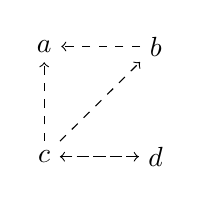
\begin{tikzpicture}
    [every node part/.style={align=center}]
    \node (a) {$a$};
    \node (b) [right = of a] {$b$};
    \node (c) [below = of a] {$c$};
    \node (d) [right = of c] {$d$};

    \draw [->, dashed] (b) -- (a);
    \draw [->, dashed] (c) -- (a);
    \draw [->, dashed] (c) -- (b);
    \draw [->, dashed] (c) -- (d);
    \draw [->, dashed] (d) -- (c);
  \end{tikzpicture}
  \caption{}
  \label{fig:abacda}
\end{wrapfigure}

Recall that earlier we said that the epistemic planning problem is decidable for
epistemic models where the preconditions and consequences of events are
\emph{propositional}. Gossip models, like those in \figref{fig:dynamicgossipex},
are an example of these\footnote{In \secref{sec:Formalisation} we show this, by
giving a way to convert between the two algorithmically.}. Due to this, we are
capable of performing planning on gossip models. In this thesis we put forward a
process with which this can be performed, and an example implementation of this.

Then given an input pair \tmc{M}, which is a gossip graph, and some formula
$\phi$ we are given the sequence of calls $c_1, c_2, \ldots, c_n$ whose
occurence on \tmc{M} will reach a state in which $\phi$ is modelled. For
example, consider the graph in Figure \ref{fig:abacda}, with the winning formula
$K_a \forall_{i \in Ag} E_i$\footnote{In this thesis we abbreviate the statement
``agent $i$ is an expert'' to be the proposition $E_i$. We also abbreviate the
statement ``all agents are experts'' to the proposition $E$, although
$\forall_{i \in Ag}E_i$ is semantically equivalent.}. Our state transition
system required by the planningThen the returned string
of calls will be $ba, ca, ad, ab, ac$. Later in this thesis we go through the
process with which this call sequence is produced, and explain the decisions
taken.  \textbf{Go over this .. weird wording}

\section{Existing Software}

As research work is done into a topic, it is only natural that software is
developed to support it. The three related pieces of software are
\cite{DEMO-S5}, \cite{SMCDEL} and \cite{GithubGossip}. These three tools are all
\emph{model checkers} for dynamic epistemic logic. A model checker is a
program that, given a model \tmc{M} and a formula $\phi$, tells the user whether
or not $\mc{M} \models \phi$. Given the setting, they specifically answer the
question ``given an initial state and a set of events, does the state reached by
the occurrence of these events at the initial state satisfy some property?''.

We can see model checking as the \emph{dual} of planning; in planning we want
to find such a sequence of events, whilst model checking verifies that these
events do indeed bring the system to a successful state. \cite{GithubGossip} is
also capable of planning, however in a na{\"i}ve way; it enumerates the set of
all possible calls and then checks if any of these are successful. As we see
later, this is a very inefficient method for planning.  

Despite this, there does not exist any software to solve the epistemic planning
problem as envisioned in the literature; indeed, the only software to solve any
epistemic planning problem is restricted to just gossip models.

\section{Contributions}

At a high level, our aim in this project is to put forward a process to solve
the planning problem for epistemic models and propositional event models. This
is motivated by the Dynamic Gossip problem; despite all of the work done in the
area of Gossip little has been done on the topic of \emph{planning} for the
Gossip problem. Dynamic Gossip can be modelled perfectly by epistemic models and
propositional event models, and hence is a perfect case study for the tool we
will develop. 

We have four major contributions in this thesis, as follows:

\begin{itemize}
\item The first contribution is the background chapter. The literature on the
  topic spans from epistemic logic to game theory, and is far outside the reach
  of the standard computer science curriculum, We present the content in a
  simple, straightforward manner, such that an undergraduate reader may
  understand all of the concepts involved.
\item Our second contribution is the derivation of an algorithm to solve the
  epistemic planning problem, as a specialisation of the sketch given in
  \cite{AutomataTechniques}. Through a scrutinization of this theory, which
  involves the very general theory of two-person games, we extract a
  conceptually clean procedure that can be understood in terms of simple
  automata theory.
\item As a testament to the functionality of the algorithm designed, we provide
  an implementation of it in Haskell. This is the first implementation of a
  planning algorithm for general epistemic models. 
\item Finally, we give an empirical evaluation of the software developed and the
  process designed. In this evaluation we inspect the correctness of the system,
  and perform a study into the program's efficiency in terms of time and space.
  As part of this, we implement a framework with which we automatically perform
  these tests. We also build a framework to aid with profiling the code.
\end{itemize}

\section{Road Map}

In Section 2, we introduce, formalise and explain the concepts and tools needed
to understand the work in the rest of the thesis. This constitutes the first of
our challenges; collecting and displaying all of the surrounding literature in a
pleasant, simple manner is a goal of this thesis and this section achieves this.

In Section 3 we put forward the algorithm we designed in order to solve the
epistemic planning problem. This uses a simplified version of the process put
forward in \secref{sec:PowersetAutomata}. We also give an exemplar execution of
the algorithm, in order to show how it functions.

Section 4 discusses the Haskell implementation of the algorithm designed in
Section 3. We discuss the design decisions taken throughout the implementation,
including motivation for the use of Haskell to solve this problem.

In Section 5 we evaluate the algorithm and its implementation. To do this we
use \cite{GithubGossip} as both a model checker, to validate our results
returned from our planning tool, and also as a tool capable of planning, in
order to analyse the space and time efficiency of our tool. 

In Section 6 we conclude the thesis. 

\newpage

\chapter{Background}

\section{Dynamic Epistemic Logic}
\label{sec:DEL}

\subsection{Epistemic Logic}

Epistemic Logic is the logical language that we use to reason about knowledge.
It is a modal logic; this is a class of logics that supplement the language of
propositional logic\footnote{By which we mean the language defined by the
  grammar $\phi ::= \top \mid p \mid \neg \phi \mid \phi \land \phi$, as well as
  the abbreviations $\bot, \lor, \rightarrow$ as is standard.} with some operator
$\boxdot$. Modal logic can be used to model the passage of time, knowledge,
obligation or any other modality. For example, $\boxdot \phi$ in temporal logic
can be read as ``at all points in the future, $\phi$ holds''; in deontic
(obligation) logic, we can read $\boxdot \phi$ as ``it is morally necessary that
$\phi$ holds''. We see that the addition of the $\boxdot$ operator provides us
with much more expressivity than the standard language of propositional logic.

In this thesis, we concern ourselves with \emph{epistemic} logic; here we
interpret $\boxdot \phi$ as ``it is known that $\phi$ holds''. However, we
change the operator slightly; we index it with the name of an agent, and we
write it as $K_i \phi$\footnote{Where the K stands for \textbf{K}nows.} Hence,
we interpret $K_i \phi$ as ``Agent $i$ knows that $\phi$ is true.''.

The essential reference on epistemic logic is \cite{ReasoningAboutKnowledge},
and it is from here that most of the information in this section comes.
  
If we have some set of agents $A$ and some set of propositions $\Lambda$, then
we define the language of epistemic logic over this set of propositions,
$\mc{L}(\Lambda)$, with the following BNF;

\begin{equation*}
  \phi ::= \top \mid p \mid \neg \phi \mid \phi \land \phi \mid K_i \phi
\end{equation*}

\noindent where $p \in \Lambda$ and $i \in A$. We can also define the dual to
$K$, in the classic way as $\widehat K_i \phi ::= \neg K_i \neg \phi$. We read
this as ``agent $i$ considers it possible that $\phi$ is true''. We can give our
epistemic logic a semantics through use of \emph{Kripke models}.

We refer to $\mc{L}(\Lambda)$ without the knowledge operator $K_i$ as
$\mc{L}_P(\Lambda)$.

\bigskip

A Kripke model $\mc{M}$ over a set of agents $I$ and a set of propositions
$\Lambda$ is a triple $(W, R, V)$, where $W$ is a set of worlds, $R$ is a set of
binary relations over $W$ indexed by an agent, such that $R_i \subseteq W \times
W$, and $V : W \rightarrow \mc{P}(\Lambda)$ is a valuation function that
associates to every world in $W$ some set of propositions that are true at it.

For epistemic logic, we think of $R_i$ as being the set of pairs of worlds that
an agent $i$ cannot distinguish between, and thus considers \emph{possible}.
This notion of epistemic possibility is essential, and is key to understanding
the rest of the thesis. As an example, consider waking up in the morning with
the curtains drawn. You cannot distinguish between the world in which it's sunny
outside and the world in which it's cloudy outside; if it were sunny outside you
could not tell, and likewise if it were cloudy outside. We label these two
worlds \Sun and \Cloud, and at this state (\Sun, \Cloud) $\in R$
\footnote{Respectively (\Cloud, \Sun) $\in R$; we later clarify that our
  relations are all symmetric.}. Hence one
considers both worlds \emph{possible}.

However when you get out of bed, open the curtains and see that it is indeed
another cloudy day in Bristol you can now distinguish between the current,
cloudy world and a world in which it is sunny - formally, (\Sun, \Cloud) $\not
\in R$. After one performs this action one no longer considers it possible that
it is sunny.

In our semantics, we use this relation to define knowledge in terms of
possibility; agent $i$ knows that something is true if it is true at all of the
worlds that $i$ cannot distinguish between.

\bigskip

When giving a semantics to a formula on a Kripke model, we need to use a
\emph{pointed Kriple model}. This is just a pair $(\mc{M}, w)$ where $w$ is a
world of $\mc{M}$. Then we read $(\mc{M}, w) \models \phi$ as ``$w$ satisfies
$\phi$''. We define the evaluation as follows:

\begin{align*}
  (\mc{M}, w) & \models \top \\
  (\mc{M}, w) & \models p \text{ iff } p \in V(w) \\
  (\mc{M}, w) & \models \neg \phi \text{ iff } (\mc{M}, w) \not \models \phi \\
  (\mc{M}, w) & \models \phi \land \psi \text{ iff } (\mc{M}, w) \models \phi \text{ and } (\mc{M}, w) \models \psi \\
  (\mc{M}, w) & \models K_i \phi \text{ iff for all $v$ such that } (w, v) \in R_i, (\mc{M}, v) \models \phi 
\end{align*}

We now shed some light on the semantics of $K_i \phi$. Recall that agent $i$
\emph{knows} a proposition to be true if it holds at all worlds $i$ cannot
distinguish from its current one. The semantics expresses this; we see that we
go to each world $v$ such that $(w, v) \in R_i$ and check that $\phi$ holds
there. This matches up with our specification, where a formula $K_i \phi$ holds
if at all indistinguishable worlds from the current one $\phi$ holds.

\bigskip 

The knowledge operator $K$ is given several properties. These are done to make
it better reflect the properties of human knowledge in the real world - thus
bringing the model closer to reality - and also in order to make it more
computationally tractable\footnote{Recall that the epistemic planning problem is
  undecidable for single-agent models with an accessibility relation which is
  not an equivalence relation.}. We make all of our relations $R_i$ equivalence
relations. This means three things;

\begin{itemize}
\item $R_i$ is \emph{reflexive}; for all $w \in W$, $(w, w) \in R_i$.
\item $R_i$ is \emph{symmetric}; for all $w, v \in W, (w, v) \in R_i$ iff $(v,
  w) \in R_i$.
\item $R_i$ is \emph{transitive}; for all $w, v, u \in W$ if $(w, v) \in R_i$
  and $(v, u) \in R_i$, then $(w, u) \in R_i$.
\end{itemize}

This is done in order to convey that agent $i$ considers world $v$ possible from
world $w$ if in both $w$ and $v$ agent $i$ has the same information; that is,
they are indistinguishable to the agent.

It is identical to say that our relations $R_i$ are equivalence relations, as it
is to say that our model is an \textsf{S5} model. This is defined as a model in
which the modal operator $K$ obeys the following axioms:

\begin{itemize}
\item \textsf{K}: $K (\phi \rightarrow \psi) \rightarrow (K \phi \rightarrow K
  \psi)$
\item \textsf{T}: $K \phi \rightarrow \phi$
\item \textsf{5}: $\widehat K \phi \rightarrow K \widehat K \phi$
\end{itemize}

These axioms hold independent of which agent's knowledge we are reasoning about. 

\bigskip \bigskip \bigskip

\begin{figure}[h]
  \centering
  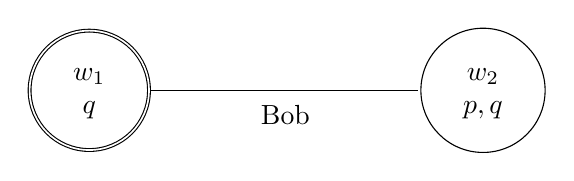
\begin{tikzpicture}
    [every node part/.style={align=center}]
    \node (1) [draw, circle, accepting] at (0, 0){
      \begin{tabular}{c}
        $w_1$ \\
        $q$
      \end{tabular}
    };
    \node (2) [draw, circle] at (5, 0) {
      \begin{tabular}{c}
        $w_2$ \\
        $p, q$
      \end{tabular}
    };

    \draw [-, shorten >= 1pt] (1) -- (2) node [midway, below = 2pt] {Bob};
  \end{tikzpicture}
  \label{fig:EgS5}
  \caption{}
\end{figure}

In Figure \ref{fig:EgS5}, we can see an exemplar Kripke Model.

In this epistemic model, we have two agents, Alice and Bob, and two worlds,
$w_1$ and $w_2$. Alice can distinguish between $w_1$ and $w_2$, and as such has
no lines on the diagram The implications of this with respect to $R_{Alice}$ are
that $(w_1, w_2) \not \in R_{Alice}$. However Bob cannot, hence the line
connecting $w_1$ and $w_2$. At $w_1$ the proposition $q$ is true, and at $w_2$
propositions $p$ and $q$ are true. Our ``actual'' world is $w_1$, and as such it
is double ringed. This means that any formula $\phi$ will be evaluated as
$(\mc{M}, w_1) \models \phi$.

To show some examples, let's evaluate some formulae on this model.

\begin{itemize}
\item $(\mc{M}, w_1) \models q$ as at $w_1$, $q$ is true.
\item $(\mc{M}, w_1) \models K_{\text{Alice}} q$. To check that this is true,
  let's consider all of the worlds Alice considers epistemically possible from $w_1$. This
  entails computing the set of worlds $\left\{ v \mid (w_1, v) \in R_{Alice}
  \right\}$. The only world is $w_1$ itself, and we know from above that
  $(\mc{M}, w_1) \models q$. Hence $K_{\text{Alice}} q$ holds here.
\item $(\mc{M}, w_1) \models \neg K_{\text{Bob}} \left( p \land q \right)$. Now
  let's consider all the worlds that Bob considers possible from $w_1$. This is
  both $w_1$ and $w_2$. But we see that $(\mc{M}, w_1) \not \models (p \land
  q)$, since $(\mc{M}, w_1) \not \models p$. 
\end{itemize}

\subsection{Event Models}
\label{sec:Event Models}

% Public announcement logic was the first development in epistemic logic to
% support \emph{information change}, and is described in \cite{PAL}. The term
% information change is quite vague; 

Public announcement logic (PAL), first described in \cite{PAL}, was the first
development in epistemic logic to support \emph{information change}. PAL
supports truthful, public communications, and supplements the language of
epistemic logic with an operator $[!\psi]$. This operator takes us to a new
model consisting of only worlds in which $\psi$ holds. For example, consider a
group of agents playing some card game. No agent knows what the others hold in
their hands; hence the set of worlds in the model is vast, as the agents
consider it possible that any player could have any card. Then agent $a$
publicly announces that he holds the 3 of spades; hence the worlds of the model
are restricted to those on which the proposition ``agent $a$ holds the 3 of
spades'' is true.

The problem with PAL is clear; we may only model truthful, public
communications. What if agent $a$ were lying, or agent $a$ was able to
communicate with agent $b$ secretively, without the other agents realising?
Clearly PAL is insufficient to model all of the complicated types of
communication that may occur. It also only is capable of modelling
communications; often, the occurence of some \emph{physical} action can change
the knowledge states of agents involved in a system\footnote{An example of this
  is given in Figure \ref{fig:cointoss}}. 

To model these more complicated events, we use \emph{event models}. These
treat events in a very similar way to how Kripke models treat worlds; we think
of a set of possible events that can occur, and encode the events that an agent
can tell apart. Just like worlds, it is possible for events to occur that an
agent cannot tell apart; for example, consider a coin being tossed, and the
result being hidden from an agent $a$. Then agent $a$ cannot distinguish between
the event in which the coin landed face up, and the event in which it landed
face down. As another example, consider a group of 4 people who can all call
each other on the phone. Agent $a$ knows that a call occurs between the other
agents, but does not know who between; hence $a$ cannot distinguish between a
call from $b$ to $c$ and $c$ to $d$, and so on. 

We give the modern definition of event models, as in
\cite{MalvinThesis}, and \cite{AutomataTechniques}, however these were first
defined in \textbf{Cite 1998 Baltag paper}

Formally, an event model \tmc{E} is a tuple $(E, P, \pre, \post)$. $E$ is a finite set
of events; $Q$ is a set of relations $Q_i$ for each $i \in Ag$, such that $Q_i
\subseteq E \times E$. As before, we make all relations $Q$ equivalence
relations. $\pre : E \rightarrow \mc{L}(\Lambda) $ is the \emph{precondition
  function}; given an event $e \in E$, it returns to us a formula that must be
true in order for $e$ to occur. $\post : E \times \Lambda \rightarrow
\mc{L}(\Lambda)$ is the \emph{postcondition function}; given an event $e \in
E$ and a proposition $p \in \Lambda$, it returns to us some formula that had to
be true at the prior state $s$ in order for $p$ to be true after event $e$
occurs at $s$. We will later give examples for these two functions. 

Updating a Kripke model \tmc{M} with an event model \tmc{E} is gives us another
Kripke model $\mc{M} \times \mc{E} ::= (W', R', V')$, where:

\begin{align*}
  W'   &::= \left\{(w, e) \in W \times E \mid (\mc{M}, w) \models \pre(e)\right\} \\
  R_i' &::= \left\{((w, e), (v, f)) \mid (w, v) \in R_i, (e, f) \in P_i, (w, e), (v, f) \in W' \right\} \\
  V'(w, e) &::= \left\{ p \in \Lambda \mid (\mc{M}, w) \models \post(e, p) \right\}
\end{align*}

We can see that the precondition function is used to ask the question ``is it
possible for the event in question to occur at the given world'', whilst the
postcondition function lets us compute the \emph{consequences} of a given event
occuring at a world. 

We should give some insight on the definition of $W'$ and $R'$. We see that in
our updated set of worlds, the worlds become pairs of elements in $W$ and events
from $E$. This will telescope infinitely; for instance worlds in $\mc{M} x
\mc{E} x \ldots x \mc{E}$ will be of the form $(\ldots (w ,e) \ldots, e)$, where
$w \in W$ and $e \in E$. Hence the worlds are traces of events that happened.
Similarly, $R'$ relates pairs of worlds from $W'$, which are again pairs of
worlds and events. Here, the worlds remain indistinguishable only if they were
indistinguishable before and both events are indistinguishable to $i$.

We see that it is the postcondition function that allows for \emph{factual
  change}; that is, the update of what is true at a state given the occurence of
some event. We can see how this gives us a much more expressive model than
simple PAL; with carefully selected \tpre and \tpost functions, we can express a
very wide range of communications and events. 

\bigskip \bigskip \bigskip

As above, we now show some example event models, and show the effects of
updating an epistemic model with an event model.

\begin{figure}[h]
  \centering
  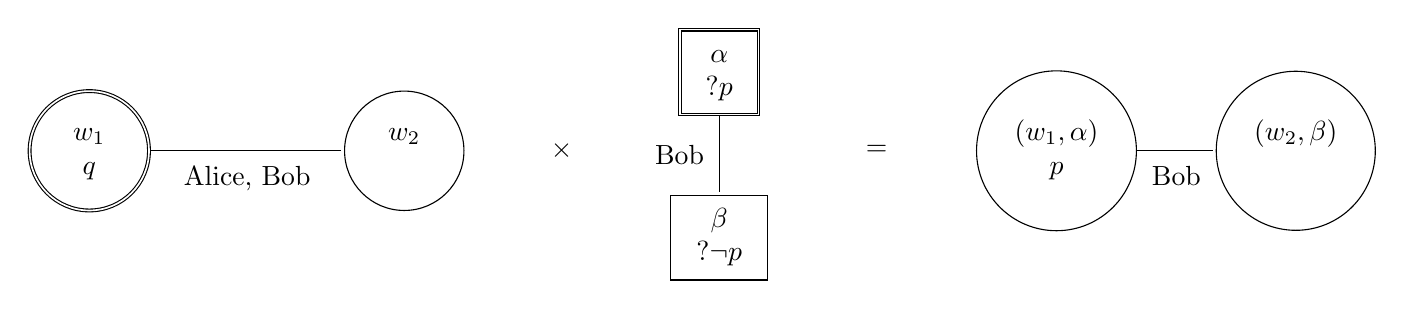
\begin{tikzpicture}
    \node(1) [draw, circle, accepting] at (0, 1) {
      \begin{tabular}{c}
        $w_1$ \\
        $q$
      \end{tabular}
    };

    \node(2) [draw, circle] at (4, 1) {
      \begin{tabular}{c}
        $w_2$ \\
        $$
      \end{tabular}
    };
    \draw[-, shorten >= 1pt] (1) -- (2) node [midway, below = 2pt] {Alice, Bob};

    \node(times) [] at (6, 1) {$\times$};
    
    \node(3) [draw, rectangle, accepting] at (8, 2) {
      \begin{tabular}{c}
        $\alpha$ \\
        $?p$
      \end{tabular}
    };
    \node(4) [draw, rectangle, below = of 3] {
      \begin{tabular}{c}
        $\beta$ \\
        $?\neg p$
      \end{tabular}
    };
    \draw[-, shorten >= 1pt] (3) -- (4) node [midway, left = 2pt] {Bob};

    \node (equals) [] at (10, 1) {$=$};

    \node(5) [draw, circle, right = of equals] {
      \begin{tabular}{c}
        $(w_1, \alpha)$ \\
        $p$
      \end{tabular}
    };
    \node(6) [draw, circle, right = of 5] {
      \begin{tabular}{c}
        $(w_2, \beta)$ \\
        $$
      \end{tabular}
    };

    \draw[-, shorten >= 1pt] (5) -- (6) node [midway, below = 2pt] {Bob};
  \end{tikzpicture}
  \caption{}
  \label{fig:PhDExample}
\end{figure}


In this example from the literature (\cite{MalvinPhD}), consider two agents,
again Alice and Bob. They are waiting in the same room to receive a letter about
Alice's entrance onto a PhD program. Suddenly the postman arrives, and Bob sees
Alice pick up and open a letter with the University's logo on the front. Alice
reads the letter and learns that she gets the position, but she does not tell
Bob the result. Bob sees that Alice now knows whether she got it, but he does
not know if she did get it or not.

Here, $p$ stands for the proposition ``Alice gets the position''. This initial
situation is represented by model \tmc{M}. In this initial situation, both Alice
and Bob cannot distinguish between the worlds where $p$ is true and where $p$ is
not true.

Then the event model \tmc{E} represents the event of Alice reading the letter
from the unviersity. $\alpha$ represents the event of Alice getting the position
and $\beta$ that she doesn't - hence the preconditions are $p$ and $\neg
p$ respectively; that is, $\pre(\alpha) = p$ and $\pre(beta) = \neg p$. Bob
cannot distinguish between either of these events, but Alice can.

Then finally the epistemic model $\mc{M} \times \mc{E}$ represents the situation
in \tmc{M} after the event \tmc{E} has occurred. We can see the epistemic model \tmc{M},
event model \tmc{E} and updated model \tmc{M \times E} in \figref{fig:PhDExample}.

\bigskip

As a second example, consider that Alice and Bob are in a room. There's a coin
on the table with the heads face up - we set this to be represented by the
proposition $p$. Alice and Bob can both see the coin face up. This situation is
modelled by epistemic model \tmc{M}.

Then Bob picks up the coin and flips it in the air. Bob sees the result of this
coin flip, but does not show Alice. We can see the event model and epistemic
model, and their update in \figref{fig:cointoss}.

Our epistemic model has just one state - that is, the state where the coin is on
the table face up. Both Alice and Bob can see the coin, and as such they both
know that $p$ holds. Then our event model has two events; $\alpha$, in which the
coin lands face-up, and $\beta$, in which the coin lands face-down. Bob can
distinguish between these two events as he can see the result of the coin toss,
but Alice cannot, because she does not see it. In the former $p$ is set to true,
and in the latter $p$ is set to false. Hence in the epistemic model $(\mc{M}
\times \mc{E})$ we have two states; that in which the coin landed face-up and
that in which the coin landed face-down.

\begin{figure}[h]
  \centering
  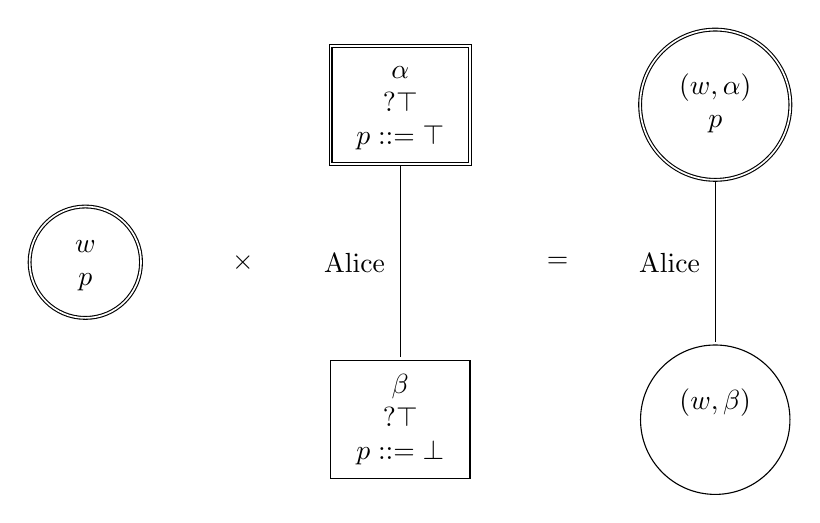
\begin{tikzpicture}
    [every node part/.style={align=center}]
    \node (0) [draw, circle, accepting] at (0, 2) {
      \begin{tabular}{c}
        $w$ \\
        $p$
      \end{tabular}
    };
    \node (1) [draw, rectangle, accepting] at (4, 4) {
      \begin{tabular}{c}
        $\alpha$ \\
        $?\top$ \\
        $p ::= \top$
      \end{tabular}
    };

    \node (times) at (2, 2) {$\times$};
    \node (2) [draw, rectangle] at (4, 0) {
      \begin{tabular}{c}
        $\beta$ \\
        $?\top$ \\
        $p ::= \bot$
      \end{tabular}
    };

    \node(3) [draw, circle, accepting] at (8, 4) {
      \begin{tabular}{c}
        $(w, \alpha)$ \\
        $p$
      \end{tabular}
    };

    \node (equals) at (6, 2) {$=$};
    
    \node(4) [draw, circle] at (8, 0) {
      \begin{tabular}{c}
        $(w, \beta)$\\
        $$
      \end{tabular}
    };

    \draw [-, shorten >= 1pt] (1) -- (2) node [midway, left = 2pt] {Alice};
    \draw [-, shorten >= 1pt] (3) -- (4) node [midway, left = 2pt] {Alice};
  \end{tikzpicture}
  \label{fig:cointoss}
  \caption{An event model and epistemic model for the coin toss example, and the
  updated event model. }
\end{figure}
    

\section{The Gossip Problem}

Gossip is a procedure for spreading secrets around a group of agents, where the
agents are commonly displayed as nodes in a graph and the ability of one agent
to contact another displayed as an edge between two nodes. Gossip was first put
forward in \cite{Tijdeman:1971}, where the network is a complete graph; all
agents can contact one another. One question here was to find how many calls are
needed for every agent to learn the secret of every other agent. We will
henceforth describe an agent knowing the secret of every other agent as this
agent being an \emph{expert}. It was quickly proved (\cite{TelephoneDisease},
\cite{GandT}) that this number, for a network where the number of agents $n$ is
greater than 4, is $2n - 4$.
 
\subsection{Dynamic Gossip}

Dynamic Gossip is a variant of the classical gossip problem, in which we start
off with an incomplete graph, representing the fact that the agents have only
the phone numbers of some of the other agents. In this case, when two agents
talk on the phone, they also exchange all of the phone numbers that they know, as
well as the secrets that they know.

\subsection{Protocols}
\label{sec:Protocols}

The gossip problem, as we have mentioned so far, can rely on some central
scheduler to tell the agents what call to make, and lets them know when to stop.
However in distributed computing, methods that do not require this central
authority are desirable. In such a situation, the agents need to have some form
of rules to follow to decide how to behave and who to call next. This is the
motivation for a \emph{gossip protocol}, which are short conditions that must
be fulfilled in order for an agent to make a specific call. These protocols were
first proposed in \cite{EPfDG}, \cite{KnowledgeandGossip}, and some exemplar
ones are:

\begin{itemize}
\item \textsf{ANY} - If $x$ knows the phone number of $y$, $x$ may call $y$.
\item \textsf{LNS} - If $x$ knows the phone number of $y$ and $x$ does not
    know the secret of $y$, then $x$ may call $y$.
\end{itemize}

In this thesis, we do not study the distributed gossip problem; rather, a
version with a central authority that surveys the network topology and then
decides which agent is allowed to make a call, and also who they will call.
However, these protocols do still have use for us. \textsf{ANY} allows for
infinite call sequences - for example, one where agent $a$ just repeatedly calls
$b$, whereas all of the call sequences induced by \textsf{LNS} are of finite
length. In the long run this does not really matter; both \textsf{ANY} and
\textsf{LNS} have runtime expected execution length in $O(n \log n)$
(\cite{DynamicGossip}), yet in our implementation tests performed with
\textsf{LNS} took considerably less time than \textsf{ANY}. For this pragmatic
reason \textsf{LNS} is often used in this thesis.

It should also be noted that there are certain classes of graphs for which
\textsf{LNS} cannot induce a successful call sequence, yet \textsf{ANY} can
(\cite{DynamicGossip}). However, this thesis does not investigate this topic,
and as such this will no longer be mentioned. 

\subsection{Formalisation}
\label{sec:Formalisation}

We now go on to formalise some of the ideas mentioned so far in this section.
The definitions of gossip graphs are classic and can be found in all of the
related literature (e.g. \cite{DynamicGossip}, \cite{MalvinThesis})

\bigskip

We formally denote a gossip graph \tmc{G} with a triple $(A, N, S)$. $A$ is a
finite set of agents in the graph; $N \subseteq A \times A$ is a set of ordered
pairs of agents such that $(u, v) \in N$ (or $Nuv$) iff $u$ knows the phone
number of $v$. $S \subseteq A \times A$ is a set of ordered pairs of agents such
that $(u, v) \in S$ (or $Suv$) iff $u$ knows the \emph{secret} of $v$.

\begin{figure}[h]
  \centering
  \begin{subfigure}[b]{0.4\textwidth}
    \centering
    \begin{tikzpicture}
      \node (a) [] at (0, 1) {$a$};
      \node (b) [] at (2, 0) {$b$};
      \node (c) [] at (3, 2) {$c$};

      \draw [<->, dashed] (a) -- (b);
      \draw [->, dashed] (b) -- (c);
    \end{tikzpicture}
    \caption{An exemplar gossip graph.}
    \label{fig:GossipSize3}
  \end{subfigure}%
  ~
  \begin{subfigure}[b]{0.4\textwidth}
      \centering
    \begin{tikzpicture}
      \node (a) [draw, rounded rectangle, accepting] {
        \begin{tikzpicture}
          \node (a) [] at (0, 1) {$a$};
          \node (b) [] at (2, 0) {$b$};
          \node (c) [] at (3, 2) {$c$};

          \draw [<->, dashed] (a) -- (b);
          \draw [->, dashed] (b) -- (c);
        \end{tikzpicture}
      };
    \end{tikzpicture}
    \caption{A Kripke model $\mc{G}$ for a Gossip State}
    \label{fig:KripkeGossip}
  \end{subfigure}
  \caption{}
  \label{fig:Gossip2Kripke}
\end{figure}


We also have that for all gossip graphs, for any agent $a$, $(a, a) \in N$ and $(a, a)
 \in S$, expressing that any agent always knows their own phone number and
 secret.

\bigskip
 
We can use the notation above to formally describe a gossip graph. For instance,
the gossip graph that we can see in \figref{fig:GossipSize3} can be expressed as
the triple $\mc{G} = (\left\{ a, b, c \right\},$ $ \left\{ (a, a), (a, b), (b, a), (b,
  b), (b, c), (c, c) \right\},$ $ \left\{ (a, a), (b, b), (c, c) \right\})$.
However given that we have the property described above, we can represent this
as the more terse $\mc{G} = (\left\{ a, b, c \right\},$ $ \left\{ (a, b), (b,
  a), (b, c)
\right\}, $ $ \left\{ \right\})$

\bigskip

One might ask how gossip fits into the picture we drew above of Kripke models
and event models. We give a way to generically define Kripke models and event
models for an arbitrary gossip graph $\mc{G} = (A, N, S)$. A Kripke model for a
graph \tmc{G} uses the set of propositions $\{N_{ij} \mid i \in A, j \in A\}
\cup \{S_{ij} \mid i \in A, j \in A\}$. We will hereafter refer to this set of
propositions as $\Lambda_{\mc{G}}$. The Kripke model for a graph \tmc{G} has
just one world, $q$, which is the world that models the graph. We define
$\mc{M_G} = (W, R, V)$ where $W = \left\{ q \right\}$, $R_i = \left\{ (q, q)
\right\}$ for every agent $i \in A$, and $V(q) = \{N _{ij} \mid (i, j) \in N\}
\cup \{S_{ij} \mid (i, j) \in S\}$. An example of this is just in
\figref{fig:Gossip2Kripke}; we see that the Kripke model for the graph is not
particularly complicated. 

An event model can also be produced in a similar way. We make an event model
$\mc{E} = (E, P, \pre, \post)$, where

\begin{itemize}
\item $E = \{ij \mid i \in A, j \in A, i \not = j\}$. Our set of events is the
  calls between agents, however an agent cannot call themself. A call is
  represented by a pair of agents; $ij$ represents a call from $i$ to $j$.
\item $P_i = \left\{(jk, j'k') \mid j, k, j', k' \in A, i \not \in \{j, k, j',
    k'\}\right\} \cup \left\{ (ij, ij) \mid j \in A\right\} \cup \left\{ (ji,
    ji) \mid j \in A \right\}$, for every $i \in A$. We can read this as agent
  $i$ cannot distinguish between a call that it is not a part of; hence the
  former part of the definition. The later two sets say that agent $i$ does not
  confuse a call that it's a part of with any other call. This means that $a$
  cannot distinguish between the world reached by the call $bc$
  happening and the world reached by the call $cd$ happening; however $a$ can
  tell the difference between worlds reached by calls it is a member of. 
\item $\pre(ij) = N_{ij}$. By this we mean that the precondition for a call from
  agent $i$ to $j$ is that $i$ knows the phone number of $j$. \\
  It is here that we
  can add in protocols from \secref{sec:Protocols}; for instance, in an event
  model where we follow the protocol \textsf{LNS}, we add the condition $\neg
  S_{ij}$ to the precondition; hence $\pre_{\textsf{LNS}}(ij) = N_{ij} \land
  \neg S_{ij}$.
\item $\post(ij, N_{nm}) = \left\{ \begin{array}{ll}
                                     N_{im} \lor N_{jm} & \text{if $n = i$ or $n =
                                                     j$} \\
                                     N_{nm} & \text{otherwise} 
                                   \end{array}
                           \right.$ \\
$\post(ij, S_{nm}) = \left\{ \begin{array}{ll}
                                     S_{im} \lor S_{jm} & \text{if $n = i$ or $n =
                                                     j$} \\
                                     S_{nm} & \text{otherwise} 
                                   \end{array}
                           \right.$ \\
 This states that if a call occurs, then for an agent $n$ to know the number of
 an agent $m$ afterwards, either $n$ was a part of the call and $n$ either knew the number
 of $m$ before or learned it from speaking to the other agent in the call, or
 $n$ was not a member of the call and knew the number of $m$ anyway. The same
 goes for secrets. 
\end{itemize}

We now give the event model for the graph \figref{fig:GossipGraph3} as an
example. 

\begin{figure}[h]
  \centering
  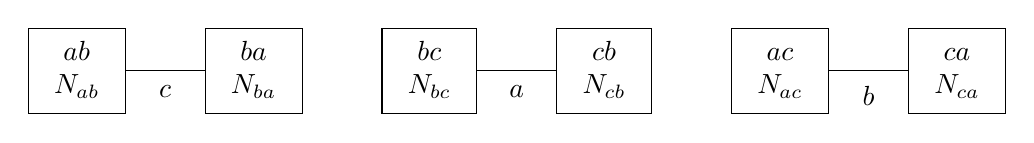
\begin{tikzpicture} [every node/.style={draw,rectangle}]
    \node (ab) [] {
      \begin{tabular}{c}
        $ab$ \\
        $N_{ab}$ 
      \end{tabular}
    };
    \node (ba) [right = of ab] {
      \begin{tabular}{c}
        $ba$ \\
        $N_{ba}$ 
      \end{tabular}
    };
    \node (bc) [right = of ba] {
      \begin{tabular}{c}
        $bc$ \\
        $N_{bc}$ 
      \end{tabular}
    };
    \node (cb) [right = of bc] {
      \begin{tabular}{c}
        $cb$ \\
        $N_{cb}$ 
      \end{tabular}
    };
    \node (ac) [right = of cb] {
      \begin{tabular}{c}
        $ac$ \\
        $N_{ac}$ 
      \end{tabular}
    };
    \node (ca) [right = of ac] {
      \begin{tabular}{c}
        $ca$ \\
        $N_{ca}$ 
      \end{tabular}
    };
    
    \draw [-] (ab) -- (ba) node [draw=none, midway, below = 2pt] {$c$};
    \draw [-] (bc) -- (cb) node [draw=none, midway, below = 2pt] {$a$};
    \draw [-] (ca) -- (ac) node [draw=none, midway, below = 2pt] {$b$};
  \end{tikzpicture}
  \caption{An Event model $\mc{E_G}$ for the calls associated with \figref{fig:GossipSize3}.}
  \label{fig:GossipEvMo}
\end{figure}

Note that this matches up with our earlier description; every agent cannot
distinguish between the calls they are not involved with. 

Recall the discussion in Section \ref{sec:Introduction}, where we say that we
choose to use the synchronous variant of the gossip problem. In this we assume
the existence of a central clock, which synchronises the calls between agents.
The implications of this are that when a call occurs, all of the other agents
are aware that a call occurs; but only the agents involved in the call are aware
of who is involved in the call. Hence when a call occurs between agents $a$ and
$b$, they know that precisely this call occured; however the other agents have
no idea which call happened; they \emph{consider it possible} that any call
between any pair of agents (excluding themselves) could have happened. 

This has implications later on in the algorithm,
but it is important to address it now. \textbf{Reference later section when we
  get there}. 

\begin{figure}
  \centering
  \begin{tikzpicture}
    \node (0) [draw, rounded rectangle] at (0, 4) {
      \begin{tabular}{c}
        $(w, ab)$ \\
        \begin{tikzpicture}
          \node (a) [] at (0, 1) {$a$};
          \node (b) [] at (2, 0) {$b$};
          \node (c) [] at (3, 2) {$c$};

          \draw [<->] (a) -- (b);
          \draw [->, dashed] (a) -- (c);
          \draw [->, dashed] (b) -- (c);
        \end{tikzpicture} 
      \end{tabular}
    };
    \node (1) [draw, rounded rectangle] at (8, 4) {
      \begin{tabular}{c}
        $(w, ba)$ \\
        \begin{tikzpicture}
          \node (a) [] at (0, 1) {$a$};
          \node (b) [] at (2, 0) {$b$};
          \node (c) [] at (3, 2) {$c$};

          \draw [<->] (a) -- (b);
          \draw [->, dashed] (a) -- (c);
          \draw [->, dashed] (b) -- (c);
        \end{tikzpicture} 
      \end{tabular}
    };
    \node (2) [draw, rounded rectangle] at (4, 0) {
      \begin{tabular}{c}
        $(w, bc)$ \\
        \begin{tikzpicture}
          \node (a) [] at (0, 1) {$a$};
          \node (b) [] at (2, 0) {$b$};
          \node (c) [] at (3, 2) {$c$};

          \draw [<->, dashed] (a) -- (b);
          \draw [<->] (b) -- (c);
          \draw [->, dashed] (c) -- (a);
        \end{tikzpicture} 
      \end{tabular}
    };

    \draw [-] (0) -- (1) node [midway, above = 2 pt] {$c$};
  \end{tikzpicture}
  \caption{The Kripke model $\mc{G} \times \mc{E_G}$.}
  \label{fig:UpdatedGossip}
\end{figure}

In \figref{fig:UpdatedGossip} we can see the result of updating the Kripke model
\tmc{G} with the event model \tmc{E_G}. We see that the call $cb$ does not have
a corresponding world; its precondition was not satisfied by any of the world in
\tmc{G}. Also note that the world $(w, ab)$ and $(w, ba)$ are indistinguishable
to $c$; this is because $c$ cannot distinguish between calls $ab$ and $ba$ as
$c$ is not included in it. Also note that the two world $(w, ab)$ and $(w, ba)$
have the exact same graph representing them\footnote{We revisit this idea of
  gossip graphs with three agents being ``boring'' again later. This
  ``boring''-ness comes from the fact that calls $ab$ and $ba$ are essentially
  the same thing.}; in the future we will not make this distinction.

In the implementation a world is represented \emph{just by the propositions that
  are true at it}. This makes use of the bijection from
$\mc{P}(\Lambda_{\mc{G}})$ to the set of gossip graphs. By this we mean that
every gossip graph (e.g. Figure \ref{fig:GossipSize3}) is represented by exactly
one set of propositions $S \subseteq \Lambda_{\mc{G}}$, and vice versa. This
gives us the useful property of being able to encode these gossip graphs with
sets of propositions in the implementation, which makes gossip graphs much easier to
deal with and reason about.

\section{Planning}
\label{sec:Planning}

Automated planning is the process of computing which set of events must occur to
take a system from some given initial state to some successful state. Such a
system is defined as a triple $\Sigma = (S, A, \gamma)$, where:

\begin{itemize}
\item $S$ is some set of states;
\item $A$ is some set of \emph{actions};
\item $\gamma : S \times A \hookrightarrow S$ is a state-transition function. It
  is partial; for $s \in S, a \in A$, either $\gamma(s, a) \in S$ or it is
  undefined. 
\end{itemize}

Then an instance of the planning problem is a triple $(\Sigma, s_i, S_g)$,
where;

\begin{itemize}
\item $\Sigma$ is a planning system;
\item $s_i \in S$ is some initial state;
\item $S_g \subseteq S$ is some set of goal states.  
\end{itemize}

A \emph{solution} to the planning problem is some ordered set of actions
${a_0, a_1, \ldots, a_n}$ such that $\gamma(\gamma(\ldots \gamma(s_0, a_0)
\ldots ,a_{n-1}) ,a_n) \in S_g$. 

Note that we call a planning problem \emph{multi-agent} if the number of
agents in the system is greater than 1, and \emph{single-agent} if the number
of agents is equal to 1. 

\subsection{Epistemic Planning}

The dynamic epistemic logic community has recently been investigating a special case
of planning, namely \emph{epistemic} planning (\cite{BolanderEP},
\cite{UndecidabilityEP}). This is planning where we may have some initial
epistemic state (e.g. agent $a$ knows $\phi$), some actions that update these
epistemic states, and some accepting epistemic state (e.g. agent $b$ knows
$\psi$). It is not hard to see how this can be applied to the gossip problem.

We give a formal definition of the epistemic planning problem that slightly
differs from convention, however with this definition and those from the
literature are equivalent. Then the epistemic planning problem is as follows;
given a pointed epistemic model $(\mc{M}, w)$ and an event model $\mc{E}$, and
some goal formula $\phi$, find some set of events ${e_1, e_2, \ldots, e_n}$ such
that $(\mc{M}, w) \otimes (\mc{E}, e_1) \otimes \ldots \otimes (\mc{E}, e_n)
\models \phi$. The \emph{propositional epistemic planning problem} is the
restriction of the epistemic planning problem to event models with pre- and
post-condition functions whose codomains are in the propositional fragment of
\tmc{L}; that is, they do not contain the modal operator $K$. These event models
are what we call propositional event models.

It is proven in \cite{BolanderEP} that the multi-agent epistemic planning
problem is undecidable for an aribtrary system. However, placing certain
restrictions on the system used yields decidability (\cite{DecidabilityEp},
\cite{AutomataTechniques}). One particularly important result is that the
propositional epistemic planning problem is decidable; indeed, it is this result
that this thesis relies on. 

% \bigskip \bigskip \bigskip

In this thesis, we focus on solving the epistemic planning problem by means of
the automata constructions described in \cite{AutomataTechniques}. These
methods, and the resulting piece of software associated with this thesis, are
unique in that they will work for any epistemic model and (propositional) event
model. This unfortunately means that we cannot plan for situations like muddy
children or drinking logicians (\cite{DEMO-S5}) as they require epistemic pre-
or post-conditions. 

The question arises of the significance of the gossip problem to the epistemic
planning problem. There are several reasons for the use of the gossip problem
as the lens through which we study epistemic planning; 

\begin{itemize}
\item It is a widely-studied problem with lots of applications already listed in
  this thesis. The consequences of this are that we have a wealth of literature
  to be used. We give examples of this in Section \ref{sec:ExistingTools}. Its
  applicability sets it apart from many other epistemic problems that are
  studied; these mainly are sorts of logic puzzles. Examples of these can be
  seen in \cite{DEMO-S5}.
\item It encapsulates very easily all of the aspects of epistemic planning that
  we're interested in - namely the indistinguishability of events from one
  another, leading to epistemic possibility from the point of view of agents -
  whilst still being a simple enough problem to understand intuitively.  
\end{itemize}

\section{Existing Tools}
\label{sec:ExistingTools}

We now give an overview of existing software in the realm of model checking or
planning for epistemic systems.

Recall that model checking for an epistemic model is the question: given an
epistemic model \tmc{M} and a formula $\phi \in \mc{L}(\Lambda)$ for some set of
propositions $\Lambda$, decide if $\mc{M} \models \phi$. Dually, planning for an
epistemic model is the question: given an epistemic model \tmc{M}, an event
model \tmc{E} and a formula $\phi \in \mc{L}(\Lambda)$ for some set of
propositions $\Lambda$, compute a sequence of events $e_1, e_2, \ldots, e_n$
where $\forall e_i$ in the sequence $e_i \in \mc{E}$ whose occurence takes the
model \tmc{M} to a state in which the formula $\phi$ is satisfied. 

\subsection{DEMO-S5}

DEMO-S5 (\cite{DEMO-S5}) is a model checker for epistemic models, limited to
$S5$ models. It is also limited in that it only supports events that are either
public announcements (e.g. an agent telling every other agent some statement) or
publicly observable factual change (e.g. the flip of a coin, where the result is
seen by every agent).

This limitation removes support for indistinguishable events; the occurence of
each event is seen by each agent and is perceived in the same way. This means
that the occurence of an event never increases the amount of worlds considered
possible by an agent; conversely, the number of worlds considered possible only
stays the same or decreases when some event occurs. This can be seen in the
``Drinking Logicians'' section of \cite{DEMO-S5}.

It performs the task of model checking by taking an epistemic model and a
formula representing either the announcement or the fact that changed, and
updating the model with the event represented by the formula. The definition of
the update used is very similar to the update of an epistemic model with an
event model as defined in Section \ref{sec:Event Models}. The given events are
applied, and at this point we check if we're in a successful state or not.

\bigskip

Unfortunately we cannot use this to model check a gossip problem, as events in
the gossip problem are neither of these; they are private one-to-one
communications. Furthermore, the software is incapable of planning; simply
checking. Despite this, the software was incredibly useful in our project in
aiding the understanding of epistemic and event models. Indeed, the
formalisation of epistemic and event models demonstrated here was used in the
code associated with this thesis.

\subsection{Gossip}

\cite{GithubGossip} is another model checker, however for strictly the gossip
problem. This program has a significant advantage over the other two pieces of
software; namely that it is capable of planning. It does this by generating all
of the possible sequences of calls on the graph and then checking which of these
are successful (i.e., after execution of all of the calls the graph is in some
successful state) and which are not. 
It also has further capabilities for
studying protocols deeply, however these are not relevant to our thesis.

Although the methods used within this software are very different to the ones
used in our implementation, this system proved to be very useful for testing
purposes, due to its simplicity of use. The results returned by our software
during testing were verified using this system. Further elaboration on this will
be given in the evaluation section of this thesis.

One limitation of this system is that is may only handle gossip states, and not
generic epistemic models. Also limiting is that it enumerates all possible call
sequences from the initial state; we are only interested in successful ones.
This means that we have the possibility of lots of wasted computation if we need
to validate lots of unsuccessful paths before we get to a successful one.

However, the biggest problem is its handling of protocols like \textsf{ANY},
which allow for infinite call sequences. The way that the call sequences is
depth-first, and the system will only check the sequences generated once they
have all been produced. This means that \textsf{ANY} it eternally generates
these call sequences, and never reaches the point at which it checks the
successful call sequences. This is clearly a big limitation and in our system we
aim to avoid this. 

\subsection{SMCDEL}

SMCDEL is the most sophisticated of the three pieces of software. A technical
report is given in \cite{SMCDEL}, whilst a lot of the underlying theory is in
\cite{MalvinThesis}. The main difference is that it uses \emph{symbolic model
  checking}, a method put forward in \cite{SymbolicModelChecking}. This gives a
much more efficient implementation \textbf{why}?, as can be seen in the
Chapter 4 of \cite{MalvinThesis}.

This software is capable of efficiently model checking all classes of epistemic
models, and also has capacity for planning; however this side of the program is
not well-displayed, and it is unclear precisely how to use it. Furthermore, due
to a reasonably unpleasant interface we choose not to use this software for
benchmarking and instead use the simpler \cite{GithubGossip}. 


\section{Uniform Strategies}
\label{sec:UniformStrategies}

Recall that in the introduction we outlined that one of our contributions was a
tool to perform epistemic planning on epistemic models and propositional event
models. So far in this chapter we have introduced the language we use to reason
about knowledge and structures with which we can model knowledge and its
dynamics. We then discussed the dynamic gossip problem, and how it can be
modelled with the techniques introduced in Section \ref{sec:DEL}, and we then
went on to introduce the planning problem. 

This background constitutes nearly everything we need to know to understand the
problem that we are solving and the process we use to do so. Section
\ref{sec:UniformStrategies} introduces \emph{uniform strategies}, to finish off
the background. Uniform strategies are the most abstract and difficult part of
this background chapter, however they end up also being the most useful tool in
our \textbf{range of tools}.

Recall that in order to verify the truth or falsity of a formula of the form
$K_i \phi$, we need to visit all the worlds that agent $i$ cannot distinguish
from their current world and see whether or not $\phi$ holds there. Doing this
quickly and easily is of great importance to our system. However, we see that in
Section \ref{sec:mestar}, this is not extremely simple to do; whilst it is
straightforward to enumerate the set of worlds that can be reached through
application of an event model to a Kripke model, it is not so straightforward to
consider the worlds that an agent may consider possible from some world. We
would need to consider the call sequence we made and compute the call sequences
that are indistinguishable to the current one. This is a slow, costly process.
What we want is to be able to evaluate epistemic formulae \emph{positionally};
that is, by only looking at the world in question.

In \cite{UniformStrategies} - the reference for uniform strategies - a process
is detailed that helps us towards this goal of positional evaluation of a
formula of form $K_i \phi$. This process takes as input an automaton \tmc{A},
whose successful states are those in which the formula $\phi$ is true, and a
transducer $\mc{T}_i$\footnote{We give a recap of transducers in Section
  \ref{sec:Transducers}.}, which relates pairs of events that are
indistinguishable to agent $i$. As output, we are returned an automata
$\widehat{\mc{A}}$ whose transitions follow those in \tmc{A}\footnote{That is,
  a word accepted by \tmc{A} will also be accepted by $\widehat{\mc{A}}$. The
  difference between the two is that the states in $\widehat{\mc{A}}$ contain
  much more information than those in \tmc{A}.}, but whose states
contain in them all of the worlds indistinguishable to agent $i$. This lets us
positionally verify formulae of the shape $K_i \phi$.

We first introduce this process - named the \emph{powerset construction} - in
the context of game arenas. These are automata-like structures, arising from
game theory, that are used in \cite{UniformStrategies} to investigate uniformity
properties of sequences of plays through graphs. In this, a modality $R$ is
introduced, meaning ``for all related plays''.

We give an overview of game arenas, a brief reintroduction to transducers and
a definition of the powerset construction. The algorithm that we later give for
epistemic planning relies heavily on this process, however uses a simplified
version. In order to illustrate that our algorithm is a special case of this
process, we introduce the powerset construction in its natural game theory
setting. 

Important to note is that this section is \emph{not} essential to understanding
the rest of this thesis. The text above details the motivation for this
technique; however the reader will be able to continue onto the next chapter
without reading the rest of this section and still understand the process very
easily. The reader may indeed get more out of this section returning to it after
reading the algorithm detailed in the next chapter. The \emph{only} part that
the reader should read is Section \ref{sec:Transducers}, which introduces our
notation used to reason about finite state transducers.

\subsection{Game Arenas}

A game with \emph{imperfect information} is a game in which the players have
some uncertainty concerning hte current configuration of the game (for example
Poker; a player does not know which cards are in the other players' hands). A
player in such a game cannot plan to play differently in a situation she cannot
distinguish; hence we have to define her strategy \emph{uniformly} across
situations she cannot distinguish. 

We consider two-player turn-based games played on a some graph, where the
vertices are labelled with propositions. These propositions hold some useful
information about the world; it could be what people know about it, or some fact
about the environment the player is in and so on. This set of propositions will
be referred to as $AP$. 

Then a game arena is a structure $\mc{G} = (V, E, v_I, l)$ where $V = V_1 \uplus
V_2$ \footnote{We use $\uplus$ here to indicate that the two sets are
  \emph{disjoint}} is a set of positions split between those of Player 1 ($V_1$)
and those of Player 2 ($V_2$). $E \subseteq (V_1 \times V_2) \cup (V_2 \times
V_1)$ is the set of edges, $v_I \in V$ is the initial position and $l : V
\rightarrow \mc{P}(AP)$ is a valuation function, which maps each position to the
finite set of propositions that are true at it.

It may be easy to see the relationship between game arenas and finite state
automata. We can see $V$ as a set of states in an automata. $E$ encodes the
transitions between states, and as such we can see it as representing the
transition function $\delta$.

\subsection{Transducers}
\label{sec:Transducers}

We give a quick recap of transducers, as they are used heavily in the next two
sections. A transducer is like a nondeterministic finite automaton with two
tapes; an \emph{input} tape and an \emph{output} tape. The transducer reads
an input finite wood on its input and writes a finite word on its output tape.
Hence a transducer defines a binary relation. Relations recognised by a
transducer are called \emph{regular} or \emph{rational} relations. 

A transducer is a 6-tuple $T = (Q, \Sigma, \Gamma, I, F, \Delta)$, where $Q$ is
a finite set of states, $\Sigma$ is the input alphabet, $\Gamma$ is the output
alphabet, $I \subseteq Q$ is a finite set of initial states, $F \subseteq Q$ is
a finite set of final states, and $\Delta \subseteq Q \times \left( \Sigma \cup
  \{\epsilon\} \right) \times \left( \Gamma \cup \{\epsilon\} \right) \times Q$
is the transition function.

$(q, a, b, q') \in \Delta$ means that the transducer can move from state $q$ to
state $q'$ by reading $a$ from the input tape and writing $b$ to the output
tape. We will use this notation throughout, however this is equivalent to saying
that $\Delta(q, a) = (b, q')$. Note that transducers are, in this thesis,
nondeterministic; hence if $\Delta = \left\{ (q, e, f, p), (q, e, g, r)
\right\}$ then $\Delta(q, e) = \left\{ (f, p), (g, r) \right\}$.

Then we can define the extended transition relation $\Delta^\ast$ as the
smallest relation satisfying:

\begin{itemize}
\item for all $q \in Q$, $(q, \epsilon, \epsilon, q) \in \Delta^\ast$
\item if $(q, w, w', q') \in \Delta^\ast$ and $(q', a, b, q'') \in \Delta$, then
  $(q, w . a, w' . b, q'') \in \Delta^\ast$
  
\end{itemize}

We can see $\Delta^\ast$ as the transitive closure of $\Delta$. We abbreviate
$(q, w, w', q') \in \Delta^\ast$ to $q \rsarrow_{w \mid w'} q'$ in the rest of
this section.

Finally, we say that the relation recognised by some transducer $T$ is

\begin{align*}
  [T] ::= \left\{ (w, w') \mid w \in \Sigma^\ast, w' \in \Gamma^\ast, \exists q_F \in F, \exists q_i \in I, q_i \rsarrow_{w \mid w'} q_F \right\}
\end{align*}

\subsection{The Powerset Arena}
\label{sec:PowersetArena}

In games with imperfect information, the \emph{information set} of a player after a
certain play is the set of positions she may possibly be in, consistent with
what she has observed\footnote{For instance in a game of poker with one deck of cards, a
player may have no idea what the other players have in their hands except that
they know they do not have the cards the player has in their own hands, nor the
cards face-up on the table.}. We can define a similar notion in our setting, and
we show that this is sufficient to build a powerset arena in which formulas of
the form $K_a \phi$, where $\phi$ is propositional, can be evaluated positionally. 

For an arena \tmc{G} and a transducer $T$ over finite sequences of events $e_i \in
E$, we construct this automata $\widehat{\mc{G}}$ in which we can evaluate
formulas of the form $K_i \phi$... 

Our new information set after a move occurs cannot be computed knowing only the
previous information set and the new position; we need to simulate the
nondeterministic execution of $T$, taking as input the sequence of positions
played and writing as output the related plays. Precisely, we need two things;
the set of states the transducer may be in after reading the sequence of
positions played so far, and for each of these states the set of possible last
positions written on the output tape. We need only remember the last letter and
not the whole tape because the information set we aim to compute is just the set
of the last positions of related plays.

Then our positions are of the form $(v, S, Last)$, where $v \in V$, $S \subseteq
Q$, where $Q$ is the set of states in the transducer and $S$ is the set of
possible current states of $T$, and $Last : S -> \mc{P}(V)$\footnote{It may be
  more helpful to think of this as something a bit more tangible than a
  function, e.g. a list of tuples $(S, [P])$} associates to a state $q \in S$
the set of the possible last positions on the output tape fo $T$ if the current
state is $q$. The transitions in this arena follow those in \tmc{G}, except we
now maintain the additional information about the configuration of the
transducer.

To construct the initial position $\widehat{v_I} = (v_I, S_I, Last_I) \in
\widehat{\mc{G}}$, we need to simulate the execution of $T$ starting from its
initial state and reading $v_I$. To do this, we introduce an artificial position
$\widehat{v_{-1}} = (v_{-1}, S_{-1}, Last_{-1})$, where $v_{-1} \not \in V$ is
some fresh position, $S_{-1} = \{q_i\}$ where $q_i$ is the initial state of the
transducer because before starting the transducer is in its initial state, and
$Last_{-1} (q_i) = \emptyset$ because we have nothing written on the output
tape.  

\bigskip

We now come onto defining \tmc{G}. Let $\mc{G} = (V, E, v_I, l)$ be an arena and
$T = (Q, V, q_i, Q_F, \Delta)$ be an FST. Then we define the arena
$\widehat{\mc{G}} = (\widehat{V}, \widehat{E}, \widehat{v_I}, \widehat{l})$ as:

\begin{itemize}
\item $\widehat{V} = V \times \mc{P}(Q) \times (Q \rightarrow \mc{P}(V))$
\item $(u, S, Last) \widehat{\rightarrow} (v, S', Last')$ if
  \begin{itemize}
  \item $u = v_{-1} \text{ and } v = v_I, \text{ or } u \rightarrow v$,
  \item $S' = \left\{q' \mid \exists q \in S, \exists \lambda' \in V^\ast, q
      \rsarrow_{v \mid \lambda'} q' \right\}$ and
  \item $Last' (q') = \left\{ v' \mid \exists q \in S, \exists \lambda' \in
      V^\ast, q \rsarrow_{v \mid \lambda' \circ v'} q', \text{ or } q \rsarrow_{v \mid
        \epsilon} q' \text{ and } v' \in Last(q) \right\}$
  \end{itemize}
\item $\widehat{v_I}$ is the only $\widehat{v} \in \widehat{V}$ such that
  $\widehat{v}_{-1} \widehat{\rightarrow} \widehat{v}$.
\item $\widehat{l}(\widehat{v}) = l (v)$ if $\widehat{v}= (v, S, Last)$. 
\end{itemize}

The definition of transitons is quite complicated, and as such we give a high-level
explanation of it. Regarding the definition of the transitions,
the first point means that our transitions in $\widehat{E}$ follow those in $E$,
except for the transition leaving $\widehat{v_{-1}}$, which we use to define
$\widehat{v_I}$. 

The second point expresses that when we move from $u$ to $v$ in \tmc{G}, we give
$v$ as input to the transducer. Then the set of states that we can be in, that
is, $S'$, is the set of states that can be reached from some previous possible
state in $q \in S$ by reading $v$ on the input tape and outputting some sequence
$\lambda'$.

Finally, the third point expresses that if some position $v'$ is at the end of
the output tape after the transducer reads $v$ and reaches $q$, then this is either
because while reading $v$ the last letter it wrote is $v'$, or it wrote nothing
and $v'$ was already at the end of the output tape before reading $v$. 

Finally, we say that $\widehat{v}_I$ is the only successor of
$\widehat{v}_{-1}$, and that the valuation of a position in the powerset arena
is the valuation of the underlying position in the original arena. 

\subsection{Lifting Transducers}
\label{sec:LiftingTransducers}

We can keep on repeating this process, creating a power-powerset arena
$\widehat{\widehat{G}}$. However we first need to lift our transducer $T$ where
$[T] \subseteq Plays_\ast \times Plays_\ast$ to a transducer $\widehat{T}$ where
$[\widehat{T}] \subseteq \widehat{Plays_\ast} \times \widehat{Plays_\ast}$.

We write $T\downarrow$ for the transducer that computers the bijective function
$f$ that maps a play $\widehat{p} \in \wh{Plays_\ast}$ to the underlying play $p
\in Player_\ast$, and $T\uparrow$ for the deterministic transducer that computes
$f^{-1}$. Both can be easily constructed from our powerset arena $\wh{G}$.

Then the lift of a transducer $T$ is $\wh{T} = T\downarrow \circ T \circ
T\uparrow$.

Once we have the transducer $\wh{T}$, we can repeat the process in Section
\ref{sec:PowersetArena} with $\wh{G}$ to get $\wh{\wh{G}}$, and so on ad
infinitum. $\wh{\wh{G}}$ would allow us to positionally check formulae of the
form $K_i K_j \phi$.

\newpage

\chapter{Algorithm}

\section{Introduction}

\begin{wrapfigure}{r}{0.2\textwidth}
  \centering
  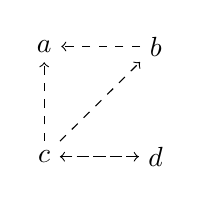
\begin{tikzpicture}
    [every node part/.style={align=center}]
    \node (a) {$a$};
    \node (b) [right = of a] {$b$};
    \node (c) [below = of a] {$c$};
    \node (d) [right = of c] {$d$};

    \draw [->, dashed] (b) -- (a);
    \draw [->, dashed] (c) -- (a);
    \draw [->, dashed] (c) -- (b);
    \draw [->, dashed] (c) -- (d);
    \draw [->, dashed] (d) -- (c);
  \end{tikzpicture}
  \caption{}
  \label{fig:introgossip}
\end{wrapfigure}

In this section, we formalise the algorithm that we use to solve the
propostional epistemic planning problem. We see this as a meaningful
contribution of the thesis; there is no existing, clear implementation of this
in the literature.

We first give a rough explanation of the process, before getting into the
details of the process later in this chapter. As part of this, we revisit the
example given in Section \ref{sec:Introduction}, to shed some light on how the
program produces the given call sequence. The gossip graph used is given in
Figure \ref{fig:introgossip}, and the successful formula in this case is $\phi =
\forall_{i \in Ag} E_i$. 

\textbf{Step one}; we receive as input an epistemic model \tmc{M}, a
propositional event model \tmc{E} and some formula $\phi \in \mc{L}(\Lambda)$,
for some set of propositions $\Lambda$. We first construct an automata called
\mestar, by simulating the repeated application of \tmc{E} onto \tmc{M}. \mestar
is a representation of all worlds that we can access from the application of any
sequence of events in \tmc{E}. This lets us easily traverse the set of possible
states we can reach from our initial model.

In the case of planning for the Dynamic Gossip problem, recall that we can
generate an event model \tmc{E} automatically given an initial gossip graph -
like the one in Figure \ref{fig:introgossip}. The gossip graph forms the model
\tmc{M}; hence given just the initial gossip graph we can produce the automata
\mestar.

Here, recall the definition of a planning problem from \secref{sec:Planning}. We
require a planning system with a set $S$ of states, a set $A$ of actions and a
partial transition function $\gamma : S \times A \hookrightarrow S$. \mestar
provides us will all of these; our set of states $S$ is the state space $Q$, the
set of actions $A$ is the alphabet $\Sigma$ and the transition function $\gamma$
is exactly the transition function $\delta$ of \mestar. Furthermore, we can
define set of goal states to be the set of states that model the winning
condition, and let the initial state be the initial state of \mestar.

\mestar when \tmc{M} is Figure \ref{fig:introgossip} and \tmc{E} is the
corresponding event model is modelled in Figure \ref{fig:introgossipE1}.


\begin{figure}[h!]
  \centering
  \begin{tikzpicture}
    \node(0) [draw, rounded rectangle] {
        \begin{tikzpicture}
          [every node/.style={draw, circle}]
          \node (a) [] {$a$};
          \node (b) [right = of a] {$b$};
          \node (c) [below = of a] {$c$};
          \node (d) [right = of c] {$d$};

          \draw[dashed, ->] (a) -- (b);
          \draw[dashed, ->] (a) -- (c);
          \draw[dashed, ->] (c) -- (b);
          \draw[dashed, <->] (c) -- (d);

        \end{tikzpicture}
      };

    \node(cb) [draw, rounded rectangle, below = of 0] {
        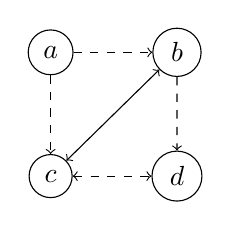
\begin{tikzpicture}
          [every node/.style={draw, circle}]
          \node (a) [] {$a$};
          \node (b) [right = of a] {$b$};
          \node (c) [below = of a] {$c$};
          \node (d) [right = of c] {$d$};

          \draw[dashed, ->] (a) -- (b);
          \draw[dashed, ->] (a) -- (c);
          \draw[<->] (c) -- (b);
          \draw[dashed, <->] (c) -- (d);
          \draw[dashed, ->] (b) -- (d);
        \end{tikzpicture}
      };

    \node(ba) [draw, rounded rectangle, left = of cb] {
        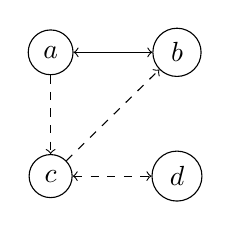
\begin{tikzpicture}
          [every node/.style={draw, circle}]
          \node (a) [] {$a$};
          \node (b) [right = of a] {$b$};
          \node (c) [below = of a] {$c$};
          \node (d) [right = of c] {$d$};

          \draw[<->] (a) -- (b);
          \draw[dashed, ->] (a) -- (c);
          \draw[dashed, ->] (c) -- (b);
          \draw[dashed, <->] (c) -- (d);

        \end{tikzpicture}
      };

      \node(dots) [right = of cb] {
        \ldots
      };

      \draw[->] (0) -- (ba) node [midway, left = 2pt] {$ba$};
      \draw[->] (0) -- (cb) node [midway, left = 2pt] {$cb$};
      \draw[->] (0) -- (dots);
    \end{tikzpicture}
    \caption{The gossip graph in Figure \ref{fig:introgossip}, updated with \tmc{E} once.}
    \label{fig:introgossipE1}
\end{figure}


\textbf{Step two}; we now consider the success formula $\phi$. If it does not
contain a knowledge modality - that is, $\phi \in \mc{L}_P(\Lambda)$ - then we
proceed to step three. However if it does (like in our example), our process
changes Recall that to find the truth value of a formula $K_i \phi$ evaluated at
some state we need to visit all of the states indistinguishable from the current
state to agent $i$ and check if $\phi$ holds at \emph{all} these states. In
\mestar we have no way of knowing which states are indistinguishable from the
state in question; hence it is very difficult to check the truth-value of such
formulae.

To this end, we perform the process detailed in Section
\ref{sec:PowersetAdapted}. In this process we build a transducer $\mc{T}_i$
which relates pairs of events that are indistinguishable to one another. We then
step through \mestar again, building another automata $\wh{\mc{ME^\ast}}$ where
the states are instead \emph{sets of states} in \mestar. This is done by
following the transitions in \mestar and, whenever we make a transition through
the occurence of an event, computing the set of events that are
indistinguishable to agent $i$ and applying this to all of the states in the set
of states that we could be in. This means that at each state in this powerset
automata, we have the set of states that $i$ considers possible, and hence we
can quickly check formulae of form $K_i \phi$. This permits \emph{positional
  evaluation} of epistemic formulae.

We can see the process of performing this procedure on the automata in Figure
\ref{fig:introgossipE1} in Figure \ref{fig:introgossipPSet}. We can see that the
calls $cb, cd$ and $dc$ all take us to the same state. This is because agent $a$
cannot distinguish between these three calls; hence the state the occurence of
any of these calls takes us to is the same. The state itself contains two state
in \mestar. The former is resulting state from applying $cb$ to the initial
state; the latter is the resulting state from applying $cd$ or $dc$ to the
initial state. Calls $ba$ and $ca$ take us to unique states. This is because
agent $i$ can distinguish between calls that they are a part of, and as such is
completely sure of which state they are in after the call occurs. 

\begin{figure}[h!]
  \centering
  \begin{tikzpicture}
    \node(0) [draw, rounded rectangle] {
        \begin{tikzpicture}
          [every node/.style={draw, circle}]
          \node (a) [] {$a$};
          \node (b) [right = of a] {$b$};
          \node (c) [below = of a] {$c$};
          \node (d) [right = of c] {$d$};

          \draw[dashed, ->] (a) -- (b);
          \draw[dashed, ->] (a) -- (c);
          \draw[dashed, ->] (c) -- (b);
          \draw[dashed, <->] (c) -- (d);

        \end{tikzpicture}
      };

    \node(cb) [draw, rounded rectangle, below = of 0] {
        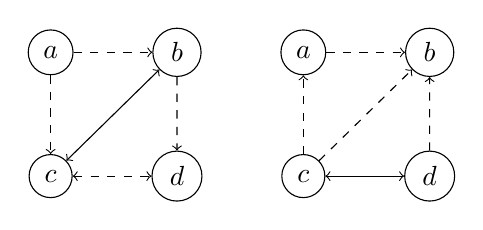
\begin{tikzpicture}
          [every node/.style={draw, circle}]
          \node (a) [] {$a$};
          \node (b) [right = of a] {$b$};
          \node (c) [below = of a] {$c$};
          \node (d) [right = of c] {$d$};
          \node (a') [right = of b] {$a$};
          \node (b') [right = of a'] {$b$};
          \node (c') [below = of a'] {$c$};
          \node (d') [right = of c'] {$d$};

          \draw[dashed, ->] (a) -- (b);
          \draw[dashed, ->] (a) -- (c);
          \draw[<->] (c) -- (b);
          \draw[dashed, <->] (c) -- (d);
          \draw[dashed, ->] (b) -- (d);

          \draw[dashed, ->] (a') -- (b');
          \draw[dashed, ->] (c') -- (a');
          \draw[dashed, ->] (c') -- (b');
          \draw[dashed, ->] (d') -- (b');
          \draw[<->] (c') -- (d');
        \end{tikzpicture}
      };

    \node(ba) [draw, rounded rectangle, left = of cb] {
        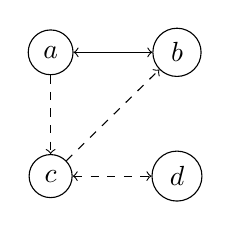
\begin{tikzpicture}
          [every node/.style={draw, circle}]
          \node (a) [] {$a$};
          \node (b) [right = of a] {$b$};
          \node (c) [below = of a] {$c$};
          \node (d) [right = of c] {$d$};

          \draw[<->] (a) -- (b);
          \draw[dashed, ->] (a) -- (c);
          \draw[dashed, ->] (c) -- (b);
          \draw[dashed, <->] (c) -- (d);

        \end{tikzpicture}
      };


    \node(ca) [draw, rounded rectangle, right = of cb] {
        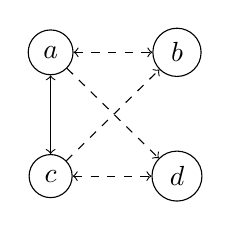
\begin{tikzpicture}
          [every node/.style={draw, circle}]
          \node (a) [] {$a$};
          \node (b) [right = of a] {$b$};
          \node (c) [below = of a] {$c$};
          \node (d) [right = of c] {$d$};

          \draw[dashed, <->] (a) -- (b);
          \draw[<->] (a) -- (c);
          \draw[dashed, ->] (c) -- (b);
          \draw[dashed, ->] (a) -- (d);
          \draw[dashed, <->] (c) -- (d);

        \end{tikzpicture}
      };
      
      \draw[->] (0) -- (ba) node [midway, left = 2pt] {$ba$};
      \draw[->] (0) -- (cb) node [midway, left = 2pt] {$cb, cd, dc$};
      \draw[->] (0) -- (ca) node [midway, left = 2pt] {$ca$};
    \end{tikzpicture}
    % \caption{Figure \ref{fig:introgossipE1}, wit}
    \caption{}
    \label{fig:introgossipPSet}
\end{figure}

We can repeat this process ad infinitum; for a formula of the form $K_b K_a
\phi$, we need to find the set of states that agents $b$ considers possible, and
then check $K_a \phi$ in these states\footnote{\label{note:KKFootnote}Note that in a situation where we have a
  formula $K_a K_a \phi$ we do not need to build another powerset automata as in
  an \textsf{S5} model, $KK \ldots KK = K$ (\cite{ModalLogic}). However, for a
  formula $K_a K_b \phi$ we do; this is because we can see $K_i$ and $K_j$ as
  being different modalities for different agents $i$ and $j$.}.

In cases where we have some conjunction or negation of formulae with a knowledge
modality in, we can just respectively perform intersection and complement on the
automata generated to solve the constituent formulae. This is a very pleasing
method and is a great display of why finite-state machines are so well-suited to
this task. 

In \textbf{step 3} we find paths through the finite-state machine we have built.
In our implementation we simply search for a single path, using breadth-first
search; however given that we have a conventional finite-state machine one could
use a wide array of other techniques to enumerate the set of all successful
paths through the automata.

After performing the breadth-first search, we either return the path found - a
string of events $e_1 e_2 \ldots e_n$ - or a negative response to say that no
path to a successful state exists. This satisfies the return requirement of a
planning problem; we return a set of actions that take us from the initial state
to some successful state, as required. 

In our example, we take the automata in Figure \ref{fig:introgossipPSet} and
search through it to find a state where the successful formula $\forall_{i \in
  Ag} E_i$ is satisfied. This is an easy task now, as we can evaluate such
formulae positionally in $\wh{\mc{ME^\ast}}$.

With this all in mind, we now move into the details of the system.

\section{\mestar}
\label{sec:mestar}

Put forward in \cite{AutomataTechniques}, \mestar is an automata we use to
represent all the worlds that can be reached and how we can move between them
given an epistemic model \tmc{M} and an event model \tmc{E}. Its name refers to
how it represents the application of \tmc{E} onto \tmc{M} infinitely. Consider
that $\mc{ME}^0$ represents $\mc{M}$, $\mc{ME}^1$ would be $\mc{M} \times
\mc{E}$, and $\mc{ME}^2$ represents $\mc{M} \times \mc{E} \times \mc{E}$, and so
on and so forth. Then we define \mestar as

\begin{equation*}
  \mc{ME}^\ast = \bigcup_{n \geq 0} \mc{ME}^n
\end{equation*}

One might wonder how we can reason about this; it's a seemingly infinite
structure. The key thing to realise is that our worlds in \mestar can be indexed
by the set of propositions that hold true at the world. This makes use of the
bijection we discussed in Section \ref{sec:Formalisation}. For instance,
\figref{fig:KripkeGossip} would be represented by the world $q_{\{N_{aa},
  N_{ab}, N_{ba}, N_{bb}, N_{bc}, N_{cc}\}}$. Recall that the set of
propositions that our epistemic model ranges over has to be finite;
consequently, our set of world is finite\footnote{Indeed, we know the exact size
  of our set of worlds in \mestar, which is $2^{|\Lambda|}$.}. The implication
of this is that two completely different call paths from the same initial world
could end at the same world in \mestar, if the sets of propositions that hold
true are the same.
\textbf{Maybe this can go? } The transitions in \mestar are exactly those from worlds in
\tmc{M} from \tmc{E}. It becomes very clear to see how this works once we
inspect the definition of \mestar.

Let $\mc{M} = (W, R, V)$ be an epistemic model, $\mc{E} = (E, \mc{R_E}, \pre,
\post)$ be an event model and $\phi \in \mc{L}_P(\Lambda)$ be a formula in
propositional logic. $\phi$ is our goal formula; we want to reach a state in
which this formula is satisfied. Then define the automaton $\mc{ME}^\ast=
(\Sigma, Q, \delta, q_i, F)$, where $\Sigma = W \cup E, F = \left\{ q_v \mid v
  \models \phi \right\}$ and $Q = q_0 \uplus \left\{ q_v \mid v \subseteq
  \Lambda \right\}$. We define $\delta$, the transition function, as follows:

\begin{centermath}
    \begin{array}{ll}
        \forall w \in W, \forall e \in E, & \\
        \delta(q_0, w) = q_{V(w)} & \delta(q_0, e) = \bot \\
        \delta(q_v, w) = \bot & \delta(q_v, e) = \left\{
            \begin{array}{ll}
                q_{v'}, \text{where } v' = \{p \mid v \models \post(e, p)\} & \text{if } v \models \pre(e) \\
                \bot & \text{otherwise.} \\
            \end{array}
        \right.
    \end{array}
\end{centermath}

\mestar is designed to accept words of the form $we_1e_2 \ldots e_n$, and such a
word is accepted if and only if

\[\delta (\ldots \delta(\delta(w, e_1), e_2), \ldots, e_n) \in F
\]

\noindent that is, all of the calls are permitted by \tpre, and the occurence of
all of the calls takes us to a world in which the winning formula is satisfied. 

We now explain the definition. We can see that our alphabet is the set of
worlds in \tmc{M} and the events in \tmc{E}. See that $\delta(q, \sigma)$ is
undefined when $q \not = q_i$ and $\sigma \in W$; we may only make a transition
when $\sigma \in W$ if $q$ is the initial world. Recall that the worlds in
\mestar are indexed just by the propositions that hold true at them; we can see
this in the definition of Q above. Then when we make a transition $\delta(q_i,
w)$ we move to the world $q_{V(w)}$, where $V$ is the valuation function from
\tmc{M}. This means that we move to the world indexed by the propositions true
at $w$.

\begin{wrapfigure}{r}{0.2\linewidth}
  \centering
  {
  \begin{tikzpicture}
      \node (a) [] at (0, 1) {$a$};
      \node (b) [] at (2, 0) {$b$};
      \node (c) [] at (3, 2) {$c$};

      \draw [<->, dashed] (a) -- (b);
      \draw [->, dashed] (b) -- (c);
    \end{tikzpicture}
    \subcaption{}
    \label{fig:GossipWrap1}
  }
  {
    \begin{tikzpicture}
      \node (a) [] at (0, 1) {$a$};
      \node (b) [] at (2, 0) {$b$};
      \node (c) [] at (3, 2) {$c$};

      \draw [<->] (a) -- (b);
      \draw [->, dashed] (b) -- (c);
      \draw [->, dashed] (a) -- (c);
    \end{tikzpicture}
    \subcaption{}
    \label{fig:GossipWrap2}
  }
  \caption{}
\end{wrapfigure}

After this, we can make no more transitions $\delta(q, \sigma)$ where $\sigma
\in W$. The only other transitions we can make are when $q \in F$ and $\sigma
\in E$. In these cases, $q$ is indexed by some set of propositions $v \subseteq
\Lambda$. Then given this, we transition to a world $q_{v'}$ where $v'$ is the
set of all propositions $p$ where the postcondition $\post(e, p)$ is modelled by
the set of propositions $v$. 

This is quite an odd definition, and we give an example to try and aid
understanding. Consider the gossip graph in \figref{fig:GossipWrap1}. In
\mestar, this would be modelled by the world $q_v$ where $v = \left\{ N_{aa},
  N_{ab}, N_{ba}, N_{bb}, N_{bc}, N_{cc}, S_{aa}, S_{bb}, S_{cc} \right\}$. When
call $ab$ occurs at \figref{fig:GossipWrap1}, \figref{fig:GossipWrap2} is the
result. We see that this matches up with the definition of $\delta$ for \mestar;
take for example $S_{ba}$. $\post(ab, S_{ba}) = S_{ba} \lor S_{aa}$ is clearly
modelled by $v$, hence this becomes true at our new world. Contrarily, consider
$S_{cb}$. $\post(ab, S_{cb}) = S_{cb}$, as $c$ is not involved in the call $ab$.
Clearly $v \not \models S_{cb}$, and as such $S_{cb}$ is not included in the set
of propositions that are true at the new world.

We also see that if the precondition of the event is not satisfied then the
world moved to is undefined; we cannot make a transition with an event that may
not happen at a world. 

\bigskip 


\section{Powerset Adapted}
\label{sec:PowersetAdapted}

In \ref{sec:PowersetArena} we give a definition of the process used construct a
powerset game arena, which constructs a super-arena in which the states of the
arena contain in them the set of states \emph{related} to the current one, given
the initial game arena and a transducer relating pairs of events. Recall the way
we compute the truth value of a formula $K_i \phi$ on some model; we find the
set of all worlds indistinguishable to $i$ from $i$'s current world and compute
the truth value of $\phi$ there.

However, \mestar is unable to perform this task. We have no way of computing the
set of indistinguishable worlds; as mentioned before, in order to compute the set
of states that $i$ considers possible we would have to go back and compute the
set of call sequences that $i$ cannot distinguish between and find the state
resulting from the application of all of these. 

It's clear to see how the powerset construction would be useful in our context;
it would give us the set of all states indistinguishable to $i$ built-in to the
states. Hence we can quickly evaluate a formula of the form $K_i \phi$ on a
state, as we have the set of indistinguishable states already built in to the
state - this is what is referred to in this thesis as \emph{positional}
evaluation. This is clearly superior to the method detailed above. 

The construction of this automata would let us perform epistemic planning when
our successful formula is of the form $K_i \phi$. Currently, with \mestar, we
may only plan where our successful formula is in $\mc{L}_P(\Lambda)$; when
planning we visit each state and evaluate the successful formula on it. We are
unable to evaluate knowledge-based formulae on states in \mestar; hence we are
unable to plan for knowledge-based formulae. The construction of a powerset
automata of \mestar - referred to as $\wh{\mc{ME^\ast}}$ - gives us this
desirable property. 

In order to perform this task we need to construct a transducer that relates
pairs of events indistinguishable from $i$. This can be built very easily from
the event model supplied, as in here these pairs are already stored. This is one
of the requisites for the powerset construction as outlined in Section
\ref{sec:PowersetArena} and refined for our use-case in Section \ref{sec:PowersetAdapted}.
In this section we give a method with which these transducers can be built, how
we compose them to make them more useful for our powerset construction, and
finally the adaptation of the powerset construction for finite state automata. 

\subsection{Event Transducers}

In conjunction with \mestar, we also need to produce a set of transducers
$\mc{T} = \{\mc{T}_i \mid i \in A\}$, for the model in question. $\mc{T}_i$
relates pairs of events that agent $i$ cannot distinguish between. This is
critical to us performing the powerset construction on our \mestar automata.
Hence we want $\left[ \mc{T}_i \right]$ to be equal to the set of pairs of calls
indistinguishable to agent $i$\footnote{As an example, consider the gossip graph
  with three agents. Then $\left[ \mc{T}_a \right] = \left\{ (ab, ab), (ac, ac),
    (ba, ba), (ca, ca), (bc, bc), (bc, cb), (cb, bc), (cb, cb) \right\} $.}.
Formally, this means that, given an event model $\mc{E} = (E, P, \pre, \post)$,
$[\mc{T}_i] = P_i$. 

In order to do this we need just one state in our transducer, which we simply
call $q$. The choice of using a one-state transducer is slightly non-standard,
however we hope it becomes clear once we see how it is used in Section
\ref{sec:TransducerComposition}. In short, we choose this because we just care
about relating hte states that are indistinguishable; the state of the model has
no impact on this \footnote{We may want to not allow a certain event because its
  precondition is not satisfied; however this is not handled in this
  transducer.}. Then given an event model $\mc{E} = (E, P, \pre, \post)$, we
define $\mc{T}_i = (\Sigma, Q, \Delta_i, q, F)$. $Q = F = \{q\}$ and $\Delta_i =
\left\{ (q, e, e', q \mid (e, e') \in P_i) \right\}$. It is quite simple to see
that this definition will satisfy the above requirement.

\subsection{Transducer Composition}
\label{sec:TransducerComposition}

Essential to this stage of the algorithm is the construction of a transducer to
relate a state with the states considered possible after some event happens by
some agent. \textbf{add example}.

This requires two components, the first of which is the transducer defined in
\ref{sec:PowersetArena}, which relates pairs of events that are
indistinguishable to an agent. This can be constructed with ease from the event
model, as discussed earlier.

The second component is the identity transducer over the automata \mestar. This
can be computed in another very straightforward manner. Given $\mc{ME}^\ast =
(\Sigma, Q, \delta, q_0, F)$, we can construct the identity transducer
$\mc{T}_{\text{id}} = (\Sigma, Q, \Delta, q_0, F)$ where $(q, e, e', q') \in
\Delta$ iff $\delta(q, e) = q'$ and $e = e'$. This is useful as it lets us
compute the effect of an event occuring and whether the event is permitted at
the world in question. The single-state transducer computes which events
\emph{could} happen, whilst the identity transducer computes the effects of
these events. 

The next step is to compose the two. We use a slightly different method than
those put forward in the literature (\cite{ComposingFSTs}), given that one of
our transducers has only one state; hence, it would not make sense to need to
move on from the state in the first transducer, as is classic. For a
single-state transducer $\mc{T}_1 = (\Sigma, \{q\}, \Delta_1, q, \{q\})$ and
a transducer $\mc{T}_2 = (\Sigma, Q, \Delta_2, q_0, F)$, we define the
composition $\mc{T} = (\Sigma, Q, \Delta, q_0, F)$ where 

\begin{align*}
  \Delta(s, e) = \left\{ (e', s') \mid (e', q) \in \Delta_1(q, e), (e', s') \in \Delta_2(s, e') \right\} 
\end{align*}

Note that \tmc{T} is nearly identical to $\mc{T}_2$; the states, alphabet,
initial and final states are the same. Recall that this is because we use
\tmc{T} to relate a world - call pair to a set of worlds that agent $i$
considers it possible to be in from the prior worlds. 

Hence, if we give as input to $\Delta$ an input pair $(q, e)$, where $q$ is a
state and $e$ an event, it returns a set of pairs of the form $(e', q')$, where
$e'$ is some event indistinguishable from $e$ and $q'$ is the state we reach
through the occurence of $e'$ at state $q$. This transducer is the one used in
the definition of the transition relation in Section \ref{sec:Powerset}.
This makes the transitions in the Powerset automata much more simple to
implement.

\subsection{Powerset}
\label{sec:Powerset}

Given an automata $\mc{ME^\ast} = (\Sigma, Q, \delta, q_i, F)$ and a transducer
$\mc{T}_i = (\Sigma, Q, \Delta, q_0, F_{\mc{T}})$, we construct a powerset
automata $\wh{\mc{ME^\ast}} = (\wh{\Sigma}, \wh{Q}, \wh{\delta}, \wh{q}_i,
\wh{F})$. In this automata, our states $\wh{q} \in \wh{Q}$ are of the form $(v,
S)$, where $S \subseteq Q$. This is because when we need to evaluate a formula
of the form $K_i\phi$, we need to know the set of states indistinguishable
to agent $i$ at this moment. The set $S$ serves this purpose; it contains all of
the states that are indistinguishable from our current state to agent $i$.

\begin{itemize}
\item $\wh{Q} = Q \times \mc{P}(Q)$
\item $\wh{\Sigma} = \Sigma$ 
\item $\wh{\delta}((v, S), \sigma) = (v', S')$ where
  \begin{itemize}
  \item $v' =  \delta(v, \sigma)$
  \item $S = \left\{q' \mid \exists q \in S, \exists \sigma' \in \Sigma,
      (\sigma', q') \in \Delta(q, \sigma) \right\}$
  \end{itemize}
\item $\wh{q}_0$ is the state $(q_0, S)$ where $S$ is the set of all worlds
  indistinguishable from $q_0$ in \mestar.
\item $\wh{F} = \left\{ (v, S) \mid v \in F \right\}$.
\end{itemize}

We see that this version is much simpler than the definition given in
\secref{sec:PowersetArena}. This is because we don't need to keep track of the
set of potential final states of the transducer's output tape; we only have to
keep track of the other possible states of the transducer. The set of states in
the transducer is exactly the same as the set of states in our \mestar automata,
so these transducer states correspond directly to the states that we
\emph{could} be in in our \mestar automata.

Note that we can update $\wh{F}$ to accept worlds in which $K_i \phi$ is made
true very easily. Assuming that in the automaton the layer below, all the states
in $F$ are those which make $\phi$ true, the definition becomes $\wh{F} =
\left\{ (v, S) \mid \forall w \in S, w \in F \right\}$\footnote{Note that given
  that we are working in an \textsf{S5} model, we know that $v \in S$. This is
  due to the \emph{reflexivity} of the accessibility relations in an \textsf{S5}
model.}.

From the definition of transitions in $\wh{\mc{ME^\ast}}$, we can see that 
$S'$ becomes the set of all states $q'$ that can be reached by making a
transducer transition with the input event $\sigma$ from some state $q \in S$.
If we recall the definition of our transducer from
\secref{sec:TransducerComposition}, a transition $\Delta(q, \sigma)$ gives
us a set of pairs $\sigma', q'$ where $\sigma'$ is some event indistinguishable
to agent $i$, and $q'$ is the state we reach from making that transition from
state $q$. 

\bigskip \bigskip \bigskip


\begin{wrapfigure}{r}{0.3\textwidth}
  \centering
  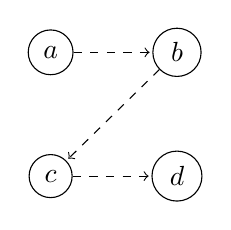
\begin{tikzpicture}
    [every node/.style={draw, circle}]
    \node (a) [] {$a$};
    \node (b) [right = of a] {$b$};
    \node (c) [below = of a] {$c$};
    \node (d) [right = of c] {$d$};

    \draw[dashed, ->, shorten >= 1pt] (a) -- (b);
    \draw[dashed, ->, shorten >= 1pt] (b) -- (c);
    \draw[dashed, ->, shorten >= 1pt] (c) -- (d);

  \end{tikzpicture}
  % \caption{An example gossip graph}
  \caption{}
  \label{fig:egGossip}
\end{wrapfigure}

We now give an example execution of this process. Consider the gossip graph in
Figure \ref{fig:egGossip}. We want to get to a state where the formula $K_a
(Sbc)$ is true; that is, we want to get to a state where agent $a$ knows that
agent $b$ knows the secret of agent $c$. One call sequence that will guarantee
this is $bc; ab$; $b$ calls $c$ to discover $c$'s secret, and then $a$ calls
$b$. At this point $a$ realises that $b$ knows the secret of $c$, and hence the
formula $K_a (Sbc)$ is satisfied. 

This is of course a very high-level description, and is unfortunately not how
the program will reason about it. Let us step through one application of the
event model \tmc{E} on this graph. In this case, our event model \tmc{E} is the
set of all possible calls, similar to Figure \ref{fig:GossipEvMo}; however only
three are permitted. The effects of updating Figure \ref{fig:egGossip} are seen
in Figure \ref{fig:egGossipE1}. We can see this as being the automata
$\mc{ME}^1$. We hope that the reader can see how the structure \mestar would
arise by repeatedly applying the event model \tmc{E} to the events in
$\mc{ME}^1$. 

\begin{figure}[h]
  \centering
  \begin{tikzpicture}
    \node(0) [draw, rounded rectangle] {
        \begin{tikzpicture}
          [every node/.style={draw, circle}]
          \node (a) [] {$a$};
          \node (b) [right = of a] {$b$};
          \node (c) [below = of a] {$c$};
          \node (d) [right = of c] {$d$};

          \draw[dashed, ->, shorten >= 1pt] (a) -- (b);
          \draw[dashed, ->, shorten >= 1pt] (b) -- (c);
          \draw[dashed, ->, shorten >= 1pt] (c) -- (d);

        \end{tikzpicture}
      };


      \node(bc) [draw, rounded rectangle, below = of 0] {
        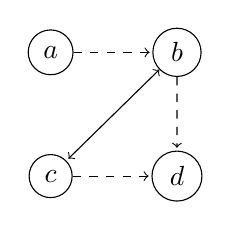
\begin{tikzpicture}
          [every node/.style={draw, circle}]
          \node (a) [] {$a$};
          \node (b) [right = of a] {$b$};
          \node (c) [below = of a] {$c$};
          \node (d) [right = of c] {$d$};

          \draw[dashed, ->, shorten >= 1pt] (a) -- (b);
          \draw[dashed, ->, shorten >= 1pt] (b) -- (d);
          \draw[<->, shorten >= 1pt] (b) -- (c);
          \draw[dashed, ->, shorten >= 1pt] (c) -- (d);
        \end{tikzpicture}
      };

      \node(ab) [draw, rounded rectangle, left = of bc] {
        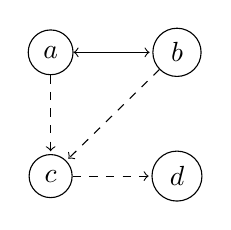
\begin{tikzpicture}
          [every node/.style={draw, circle}]
          \node (a) [] {$a$};
          \node (b) [right = of a] {$b$};
          \node (c) [below = of a] {$c$};
          \node (d) [right = of c] {$d$};

          \draw[<->, shorten >= 1pt] (a) -- (b);
          \draw[dashed, ->, shorten >= 1pt] (a) -- (c);
          \draw[dashed, ->, shorten >= 1pt] (b) -- (c);
          \draw[dashed, ->, shorten >= 1pt] (c) -- (d);

        \end{tikzpicture}
      };
      
      \node(cd) [draw, rounded rectangle, right = of bc] {
        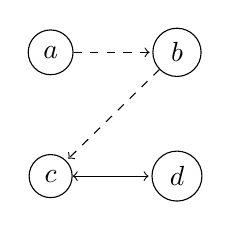
\begin{tikzpicture}
          [every node/.style={draw, circle}]
          \node (a) [] {$a$};
          \node (b) [right = of a] {$b$};
          \node (c) [below = of a] {$c$};
          \node (d) [right = of c] {$d$};

          \draw[dashed, ->, shorten >= 1pt] (a) -- (b);
          \draw[dashed, ->, shorten >= 1pt] (b) -- (c);
          \draw[<->, shorten >= 1pt] (c) -- (d);
        \end{tikzpicture}
      };

      \draw[dashed, ->, shorten >= 2pt] (0) -- (ab) node [midway, left = 2pt] {$ab$};
      \draw[dashed, ->, shorten >= 2pt] (0) -- (bc) node [midway, left = 2pt] {$bc$};
      \draw[dashed, ->, shorten >= 2pt] (0) -- (cd) node [midway, left = 2pt] {$cd$};
      \draw[-, red] (bc) -- (cd) node [midway, below = 2pt] {$~_a$};
    \end{tikzpicture}
    \caption{The gossip graph in \ref{fig:egGossip}, updated with \tmc{E} once.}
    \label{fig:egGossipE1}
\end{figure}

\bigskip 

Figure \ref{fig:egGossipE1} shows the three possible states that we could be in
afer making one call from the initial state displayed in Figure
\ref{fig:egGossip}. The red line indicates that agent $a$ cannot distinguish
between these two states, as they were both reached by the execution of a call
that agent $a$ was not a member of. Note that in the algorithm this connection
does not exist; it's here simply for labelling. We can see the three states on
the lower row as a Kripke model, where the three are worlds labelled by their
valuation, and the two connected by the red line are indistinguishable to $a$.

Now say that we wanted to evaluate the formula $\neg S_{ba}$ on the bottom-right
world in Figure \ref{fig:egGossipE1}. This is very straightforward; we just need
to check if $b$ does indeed know $a$'s secret; here it doesn't, and so the world
satisfies $\neg S_{ba}$. But what if we want to evaluate the formula $K_a \neg
S_{ba}$? We need to visit each of the states indistinguishable from the state in
question and see if $\neg S_{ba}$ holds there. Recall that, although
the red line connecting the two bottom states indicates that agent $a$ cannot
distinguish between these two worlds, this connection \emph{does not exist} in
the automata; it is there just for our intuitions. \mestar has \emph{no notion}
of two states being indistinguishable from one another.

Hence, this is currently impossible; \mestar has no idea whether agent $a$
cannot distinguish between this world and any others, and certainly no way of
reaching such worlds. This is where the powerset construction comes into play;
we pull the indistinguishable states into the states themselves, yielding the
possibility for \emph{positional evaluation} of $K_a \neg S_{ba}$. Hence, Figure
\ref{fig:egGossipE1} becomes Figure \ref{fig:egGossipE1pset}.

\begin{figure}[h]
  \centering
  \begin{tikzpicture}
    \node(0) [draw, rounded rectangle] {
        \begin{tikzpicture}
          [every node/.style={draw, circle}]
          \node (a) [] {$a$};
          \node (b) [right = of a] {$b$};
          \node (c) [below = of a] {$c$};
          \node (d) [right = of c] {$d$};

          \draw[dashed, ->, shorten >= 1pt] (a) -- (b);
          \draw[dashed, ->, shorten >= 1pt] (b) -- (c);
          \draw[dashed, ->, shorten >= 1pt] (c) -- (d);

        \end{tikzpicture}
      };

      \node(btwn1) [below = of 0] {};

      \node(btwn) [below = of btwn1] {};

      \node(ab2) [draw, rounded rectangle, left = of btwn] {
        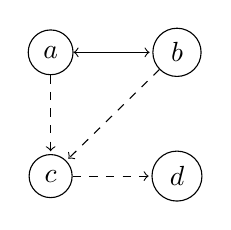
\begin{tikzpicture}
          [every node/.style={draw, circle}]
          \node (a) [] {$a$};
          \node (b) [right = of a] {$b$};
          \node (c) [below = of a] {$c$};
          \node (d) [right = of c] {$d$};

          \draw[<->, shorten >= 1pt] (a) -- (b);
          \draw[dashed, ->, shorten >= 1pt] (a) -- (c);
          \draw[dashed, ->, shorten >= 1pt] (b) -- (c);
          \draw[dashed, ->, shorten >= 1pt] (c) -- (d);

        \end{tikzpicture}
      };
      
      \node(cd) [draw, rounded rectangle, right = of btwn] {
        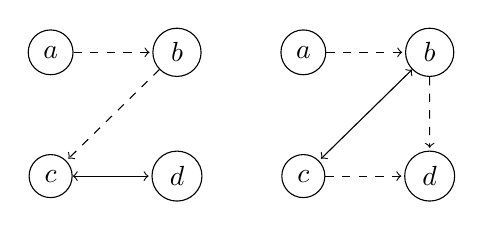
\begin{tikzpicture}
          [every node/.style={draw, circle}]
          \node (a) [] {$a$};
          \node (b) [right = of a] {$b$};
          \node (c) [below = of a] {$c$};
          \node (d) [right = of c] {$d$};

          \node (aa) [right = of b] {$a$};
          \node (ab) [right = of aa] {$b$};
          \node (ac) [below = of aa] {$c$};
          \node (ad) [right = of ac] {$d$};


          \draw[dashed, ->, shorten >= 1pt] (a) -- (b);
          \draw[dashed, ->, shorten >= 1pt] (b) -- (c);
          \draw[<->, shorten >= 1pt] (c) -- (d);

          \draw[dashed, ->, shorten >= 1pt] (aa) -- (ab);
          \draw[dashed, ->, shorten >= 1pt] (ab) -- (ad);
          \draw[<->, shorten >= 1pt] (ab) -- (ac);
          \draw[dashed, ->, shorten >= 1pt] (ac) -- (ad);

        \end{tikzpicture}
      };

      \node(bc) [draw, rounded rectangle, below = of btwn] {
       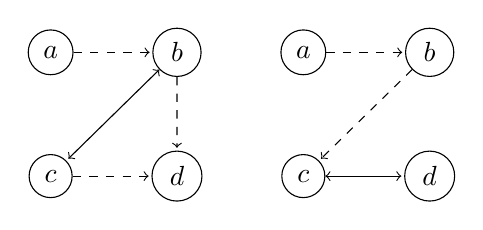
\begin{tikzpicture}
          [every node/.style={draw, circle}]
          \node (a) [] {$a$};
          \node (b) [right = of a] {$b$};
          \node (c) [below = of a] {$c$};
          \node (d) [right = of c] {$d$};

          \node (aa) [right = of b] {$a$};
          \node (ab) [right = of aa] {$b$};
          \node (ac) [below = of aa] {$c$};
          \node (ad) [right = of ac] {$d$};


          \draw[dashed, ->, shorten >= 1pt] (aa) -- (ab);
          \draw[dashed, ->, shorten >= 1pt] (ab) -- (ac);
          \draw[<->, shorten >= 1pt] (ac) -- (ad);

          \draw[dashed, ->, shorten >= 1pt] (a) -- (b);
          \draw[dashed, ->, shorten >= 1pt] (b) -- (d);
          \draw[<->, shorten >= 1pt] (b) -- (c);
          \draw[dashed, ->, shorten >= 1pt] (c) -- (d);

        \end{tikzpicture}
      };


      \node(ab3) [draw, rounded rectangle, below = of bc] {
       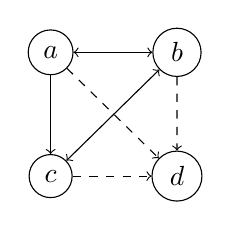
\begin{tikzpicture}
          [every node/.style={draw, circle}]
          \node (a) [] {$a$};
          \node (b) [right = of a] {$b$};
          \node (c) [below = of a] {$c$};
          \node (d) [right = of c] {$d$};

          \draw[<->] (a) -- (b);
          \draw[->] (a) -- (c);
          \draw[dashed, ->] (a) -- (d);
          \draw[dashed, ->] (b) -- (d);
          \draw[<->] (b) -- (c);
          \draw[dashed, ->] (c) -- (d);

        \end{tikzpicture}
      };
      
      \draw[dashed, ->] (0) -- (ab2) node [midway, left = 2pt] {$ab$};
      \draw[dashed, ->] (0) -- (bc) node [midway, left = 2pt] {$bc$};
      \draw[dashed, ->] (0) -- (cd) node [midway, left = 2pt] {$cd$};
      \draw[dashed, ->] (bc) -- (ab3) node [midway, left = 2pt] {$ab$};
    \end{tikzpicture}
    \caption{The automata in Figure \ref{fig:egGossipE1}, now with the
      indistinguishable states in the states.}
    \label{fig:egGossipE1pset}
\end{figure}

The difference between Figures \ref{fig:egGossipE1} and \ref{fig:egGossipE1pset}
now is that the former has all of the states indistinguishable to itself inside
the state. This means that we can evaluate the formula $K_a \neg S_{ba}$ at a
state by simply inspecting the states indistinguishable from the one we're
looking at to check a formula of such form. This is now an extremely
straightforward task! 

In Figure \ref{fig:egGossipE1pset} we display the \emph{true} state on the left.
This is the state that contains the true information of the state reached by
making the corresponding call. This is very important, as when an agent calls
another they become aware of the knowledge state of the other. To revisit the
example from the start of this section, consider again the formula $K_a (Sbc)$.
Recall that we said a successful call sequence would be $bc, ab$. Observe that
in the state reached from the initial state by the call $bc$ in Figure
\ref{fig:egGossipE1pset} there are two states that cannot be distinguished
between by $a$. However, upon the event of $a$ calling $b$, $a$ learns that $b$
knows the phone number of $c$ - this is the \emph{underlying} state that we talk
about. Hence the state at the bottom of Figure \ref{fig:egGossipE1pset} contains
only one possible world; $a$ no longer considers the other possible, as the
knowledge of $b$ is different. Happily, this leads us to a state in which $K_a
Sbc$ is satisfied, just as we promised. 

\section{Combining Automata}

When we encounter a formula of the form $\phi \land \psi$, where $\phi, \psi \in
\mc{L}_P(\Lambda)$, we can simply apply the method described in Section
\ref{sec:mestar} to produce an automata whose successful states are those in
which $\phi \land \psi$ are made true. The production of an automaton whose
successful states are those in which a formula $\chi$ is made true is a process
that we call \emph{constructing an automata to solve $\chi$}.

However this is less straightforward when we encounter a formula of the formula
$K_a \phi \land K_b \psi$ \footnote{This occurs very frequently; in this gossip
  problem, we often want to reach a state where every agent knows that everyone
  is an expert.}; in this case, we want to produce powerset automata for $K_a
\phi$ and $K_b \phi$ and then join them back up somehow.

Luckily, intersection for finite automata is well-defined. We give the
definition here. For two automata $A = (\Sigma, Q_A, \delta_A, q_{0A}, F_A)$, $B
= (\Sigma, Q_B, \delta_B, q_{0B}, F_B)$, we define their intersection $A \cap B =
(\Sigma, Q, \delta, q_0, F)$ where $Q = Q_A \times Q_B$, $F = F_A \times F_B$,
$q_0 = (q_{0A}, q_{0B})$ and $\delta(q_A, q_B) = (\delta_A(q_A), \delta_B(q_B))$.

This definition expands in the simple way when we want to take the conjunction
of $n$ automata. 

\bigskip

We have a similar story for negation; given a formula $\neg K_a \phi$, to create
an automata to solve this we build the automata to solve $K_a \phi$ and then
take the complement of this. This consists of simply changing the set of
accepting states. Given automata $A = (\Sigma, Q, \delta, q_0, F)$, we define
$A_\neg = (\Sigma, Q, \delta, q_0, F_\neg)$ where $F_\neg = Q \setminus F$.

\bigskip

To complete our little family of set operations, we should define disjunction
too. Taking the union of automata is, algorithmically, less straightforward than
the intersection; hence we just exploit de Morgan's law and use the identity $A
\cup B = (A^C \cap B^C)^C$. We recognise that when we come to implementation
this may be more costly than some alternative implementation, but for now this
is of little importance. 

\section{Searching}

Then given our solving automata, we want to traverse it to find paths that takes
us from the initial state to some successful state. It is in here that the
process of planning is really performed; everything up to this point has been
merely preparation for this. 

In this stage, we simply view the automata as a \emph{directed graph} and
perform breadth-first search on the automata. Each of the edges are weighted
equally\footnote{If we had some situation where certain communication channels
  were more expensive or slower in a network, we could emulate this by making
  some of the edges weighted.}. This way we find the \emph{shortest path} from
the root note to one of the final nodes. This is one reason why breadth-first
search was chosen over depth-first; another is that it breadth-first search is
less prone to one of the pitfalls of \cite{GithubGossip}, which is that it can
infinitely loop sometimes when using a gossip protocol like \textsf{ANY}.
Protocols like \textsf{ANY} can allow for infinite call sequences. A depth-first
search strategy will result in the searching of infinite call sequences; this
means that the program will loop infinitely and never return. With a
breadth-first search this is less likely to happen, although in the case of
there being no successful state in the graph this is still possible. To remedy
this we pre-process the automata to remove all transitions from a state to
itself. This means that there is no scope to repeatedly investigate a state. 

% Recall our earlier definition of \mestar. We can see \mestar as being the
% repeated application of some event model \tmc{E} onto some epistemic model
% \tmc{M}. Hence, we can see \mestar as being structures similarly to Figure
% \ref{fig:mestarStructure}; each time we perform a call we travel further down
% the 

% \begin{figure}[h]
%   \centering
%   \begin{tikzpicture}[every node part/.style={align=center}]
%     \node(0) [draw, rounded rectangle] at (0, 4) {Nodes in $\mc{ME}^0$};
%     \node(1) [draw, rounded rectangle] at (0, 2) {Nodes in $\mc{ME}^1$};
%     \node(2) [draw, rounded rectangle] at (0, 0) {Nodes in $\mc{ME}^2$};
%     \node(3) at (0, -2) {\ldots};

%     \draw[->, shorten >= 1pt] (0) -- (1) node [midway, left = 3pt] {Calls in \tmc{E}};
%     \draw[->, shorten >= 1pt] (1) -- (2) node [midway, left = 3pt] {Calls in \tmc{E}};
%     \draw[->, shorten >= 1pt] (2) -- (3) node [midway, left = 3pt] {Calls in \tmc{E}};
%   \end{tikzpicture}
%   \caption{}
%   \label{fig:mestarStructure}
% \end{figure}

% After any kind of powerset, intersection or complement operation, it will still
% follow the same shape; we have layers, and as they get deeper more events get
% applied to them. One big benefit of this topology is that the resultant graph is
% \emph{acyclic}; there is no way we can return to an earlier state.

% This is one of the reasons that a breadth-first traversal of the resultant graph
% is most suitable for this context. 

\newpage 

\chapter{Implementation}

We now come to covering the implementation of the algorithm developed in the
previous chapter. We will first give an overview of the structure of the
software and then a summary of all design decisions taken throughout. 

For the implementation of our algorithm, we chose to use Haskell. Haskell is a
lazy functional programming language, which gives us several benefits for this
particular task that other languages lack. 

The first one is the syntax; its functional style lends itself very well to
mathematical definitions. Its list comprehension and pattern matching let us
write code that very closely mimics the original notation, thus erasing a lot of
the difficulty of converting a mathematical definition to code once we have
implemented it. 

Another benefit is its laziness. In our implementation we often use automata
with a ridiculously large state space; however (thankfully) Haskell's laziness
means that we never have to enumerate these states. We only need to access them
when we need them. This saves a lot of processing time, as well as greatly
reduces the space the program takes up.

Its strong type system and typeclasses support us and give us safety guarantees,
preventing us from writing erroneous code that in another language may only be
detected at runtime. A simple example is that in our implementation we cannot
represent a formula that is not well-formed; a more sophisticated one is the
ability to make sure that an epistemic model and an event model span the same
set of atomic propositions and events. Typeclasses help us make code that is
very reusable but also safe; if we wanted to use a new language of atomic
propositions for an existing model, we would only need to give an instance of
the \mih{Prop} typeclass for our new language and hey presto.

The classification of functions as first-class objects also comes in very
helpful. In the implementation we make the transition function of an FSM a
function $\delta : Q \times \Sigma \rightarrow Q$. Often we want to ``lift'' the
states $Q$ to some other data type, e.g. $P (Q)$. We can very easily unwrap the
datatype $P$ to access the underlying $Q$ and then use the previous $\delta$
function; this would be much more tricky in a language other than Haskell,
however in Haskell it is a very pleasant thing to do.

Haskell offers a simple way to divide each file into a module and import (or
not) a module into another. We give a brief overview of each module in the
system, and highlight notable uses of any of the above language features in this
process. We also highlight any notable design choices made.

All of the code discussed in this section and associated with this thesis can be
found at \url{https://github.com/leopoulson/gossip-planning}. In the code
samples in this thesis we often remove or shorten certain functions in order to
better display the aspects of the code we \emph{want} to show, and remove the
irrelevant clutter. 

\section{\mih{Model.hs}}

This section is arguably the foundation of the system. Here we implement the
structures defined in \secref{subsec:DEL}; we have the language of our formulae,
Kripke models, Event models and updates thereof.  

In Figure \ref{fig:HaskellModels}, we can see the implementation of both Kripke
models and event models in Haskell. \mih{states} and \mih{events}
respectively represent the states and events of the Kripke and Event models, and
\mih{eprel} and \mih{evrel} respectively represent the
indistinguishability relations between them. Note that for ease of
implementation we use \emph{partitions} (\cite{EREL}) of sets rather than sets
of pairs. This is done because we regularly want to just access the set of
states we cannot distinguish an item between, and the use of partitions makes
this a much simpler task. 

\begin{figure}[h]
  \centering
  \begin{subfigure}[b]{0.5\textwidth}
    \begin{minted}{haskell}
      data EpistM ev prp = Mo {
        states :: [State ev],                  
        agents :: [Agent],              
        val :: [(State ev, [Form prp])],         
        eprel :: [(Agent, [[State ev]])],
        actual :: [State ev],              
        allProps :: Set prp
      }
    \end{minted}
    \caption{The Kripke model datatype}
  \end{subfigure}%
~
  \begin{subfigure}[b]{0.5\textwidth}
    \begin{minted}{haskell}
      data EventModel ev prp = EvMo {
        events :: [ev],
        evrel :: [(Agent, [[st]])],
        pre :: ev -> Form prp,
        post :: (ev, prp) -> Form prp
      }
    \end{minted}
    \caption{The Event model datatype}
  \end{subfigure}
  \caption{}
  \label{fig:HaskellModels}
\end{figure}

In Figure \ref{fig:HaskellModels} we see the first leverage of Haskell's type
system. Through making our models parametric in the propositions of the language
used (formally referred to as $\Lambda$) and the events used. These parameters
mean that when we use them in a function they necessarily use the same events
and propositions. Consider the function signature for \mintinline{haskell}{update}.
% \mintinline{haskell}{update:: Prop p => EpistM ev p -> EventModel ev p -> EpistM
% ev p}.

\begin{figure}[h]
  \centering
  \begin{minted}{haskell}
    update :: Prop p => EpistM ev p -> EventModel ev p -> EpistM ev p
\end{minted}
  \caption{}
  \label{fig:UpdateType}
\end{figure}

If we try and use the \mintinline{haskell}{update} function with models using
different types of events or propositions we get a compiler error. This type
safety, and ease of use of it, is one of the main attractions of Haskell for
this project, giving us a type-safety unavailable in a language like C.

One may also notice in Figure \ref{fig:UpdateType} the use of the typeclass
\mih{Prop p}. This typeclass guarantees us a function
\mintinline{haskell}{evalState :: p -> EpistM st p -> st -> Bool}, which given a
model, propositions and a state within the model, returns a boolean value
expressing whether or not the proposition in question holds at the state. This may
seem nonsensical - given that we have no information about what the state is
from the type, we can not do anything too interesting - however it becomes
useful in the case of propositions like $N_{ii}$; an agent will always know
their own phone number. 

The user then defines their own \tpre- and \tpost-condition functions. One
deviation from the mathematical notation is the addition of the set of agents;
this is purely a pragmatic thing, as it makes certain operations more
straightforward later on.

\begin{figure}[h]
  % \centering
  \begin{subfigure}[b]{0.5\textwidth}
  \begin{minted}{haskell}
    update :: (Eq ev, Prop p) => EpistM ev p -> EventModel ev p -> EpistM ev p
    update epm evm = Mo states' (agents epm) val' rels' (actual epm) (allProps epm)
      where
        states' = [stateUpdate s ev | s <- states epm, ev <- events evm, satisfies (epm, s) (pre evm ev)]
        rels' = [(ag, newRel ag) | ag <- agents epm]
        newRel agent = filterRel states' [liftA2 stateUpdate ss es |
                                          ss <- fromMaybe [] (lookup agent $ eprel epm),
                                          es <- fromMaybe [] (lookup agent $ evrel evm)]
        val' = [(s, ps s) | s <- states']
        ps s = [P p | p <- props, satisfies (epm, trimLast s) (post evm (lastEv s, p))]
        props = allProps epm
  \end{minted}
\end{subfigure}
\caption{The $\mc{M} \times \mc{E}$ function}
\label{fig:update}
\end{figure}

Now we see the definition for the update of a Kripke model with an event model.
Whilst the agents, set of propositions and actual world remain the same, we
update the states, epistemic relations and valuation function in a way very
similar to the definition in \secref{subsec:EventModels}. This is a display of
the merits of Haskell; our implementation stays very close to the specification,
allowing for simple visual verification that the code that we've written matches
the specification. 

\section{\mih{FSM.hs} and \mih{FST.hs}}

These two modules hold our finite state machines. Given how much of the
algorithm relies on state machines, it was very important in development to have
a reliable structure for state machines. Furthermore, we needed to do some
non-standard operations on the machines we implemented (namely, the composition
mentioned in \secref{sec:TransducerComposition}). To do this easily we need
low-level access to the states and a good understanding of the library. 

The two libraries that seemed most suitable were \cite{HaskellFST} and
\cite{HaskellMachines}. However, both libraries carried complexity unnecessary
for our use-case; furthermore it was particularly unclear how we would go
about implementing our single-state composition as mentioned above. 

Fortunately, implementation of these finite-state machines is incredibly
straightforward. We can see in \figref{fig:FSMFST} that the datatypes nearly
identically mimic the tuple definitions in \secref{sec:Transducers}.


\begin{figure}[h]
  \centering
  \begin{subfigure}[b]{0.5\textwidth}
    \begin{minted}{haskell}
      data FSM ch st = FSM {
        alphabet :: [ch],              
        states :: [st],               
        transition :: (st, ch) -> Maybe st,
        initial :: [st],            
        accepting :: st -> Bool    
       }
    \end{minted}
    \caption{The FSM datatype}
  \end{subfigure}%
~
  \begin{subfigure}[b]{0.5\textwidth}
    \begin{minted}{haskell}
      data FST ch st = FST {
        alphabet :: [ch],                     
        states :: [st],                       
        bitransition :: (st, ch) -> [(ch, st)],
        initial :: [st],                      
        accepting :: st -> Bool              
      }
    \end{minted}
    \caption{The FST datatype}
  \end{subfigure}
  \caption{}
  \label{fig:FSMFST}
\end{figure}

Our FSM's transition returns a \mih{Maybe st} to encode that it is
\emph{nondeterministic}; meaning that it is not guaranteed to return a state
on a transition. This comes in useful in practise when we have as input to
$\delta$ some pair $(w, e)$ where $e$ is not permitted at $w$. In this case,
$\delta(w, e) = \text{\mih{Nothing}}$. An example of this is a call $ij$ in the
gossip problem where $i$ does not know $j$'s phone number.

Similarly, the FST transition returns a list of $(e, q)$ pairs. This again
encapsulates the nondeterminism of the FST. This is useful in the case of
\secref{sec:TransducerComposition}, where we want to return from
$\Delta(q, e)$ the set of all pairs $(e', q')$ where $e'$ is some event
indistinguishable from $e$ and $q'$ is the state reached by making the
transition $\delta(q, e')$.

A decision we made in the design of the machines was the encoding of transitions
as \emph{functions}, rather than as a map. We chose to do this for a number of
reasons. Firstly, we never wish to enumerate the set of transitions in the
graph, a task which is made easier through the use of maps. Further, use of a
map requires us to ``be strict in our keys, but lazy in the values''
(\textbf{cite hackage page}). Although better than being strict in keys and
values, this is still quite unpleasant; consider \mestar. We want to be able to
mimic from every state to every other, even the impossible states\footnote{We
  can imagine an ``impossible'' state as a state that we would never reach in
  the model. For example, in the gossip problem, an impossible state would be
  one in which everyone knows everyone else's secret, but no one knows anyone
  else's phone number.}. When using a Map, this would mean we would require an
entry for all of these impossible state. This means that a lot of time would be
spent on entering keys into the map for states that \emph{will never be used}.
However, when we use a function, these inputs are covered for free. This is a
much easier way to handle transitions. A similar argument holds for the
\mintinline{haskell}{accepting} function. 

The use of functions here is a method that can only be easily utilised in
languages where functions are treated as first-class objects (Haskell is one of
these). This treatment of functions also makes operations like intersection and
complement of FSMs a simplicity; in the latter case, we simply need to compose
the \mintinline{haskell}{not} function before the accepting function. 

\section{\mih{ME.hs}}
\label{sec:MEHaskell}

\begin{wrapfigure}{r}{0.3\textwidth}
  \begin{minted}{haskell}
    class (Ord st, Prop p) => EvalState st p where
      evalState :: Form p -> st -> Bool
\end{minted}
  \caption{}
  \label{fig:EvalState}
\end{wrapfigure}

We now come onto the module that handles construction of the automata \mestar.
This is a slightly more interesting case.

In this module we make use of one of the many language extensions Haskell offers
us, namely \mih{MultiParamTypeClasses}. This gets around the limitation that
GHC enforces of being unable to use a typeclass with more than one type
parameter, allowing us to write typeclasses like this in Figure
\ref{fig:EvalState}.

This lets us ensure in our functions that the propositions we're using can be
evaluated at the states we want them to be evaluated at. This prevents us from
trying to evaluate formula of a certain language on a world it is incompatible
with. This is another display of the way we can use Haskell's type system to our
advantage. 

\begin{figure}[h]
\begin{minted}{haskell}
meTrans :: (Prop p, Eq ev) => EpistM ev p -> EventModel ev p -> ((QState p, ev)
-> Maybe (QState p))
meTrans (Mo _ _ _ _ _ props) evm    (Q ps, ev)
    | not $ ps `models` pre evm ev  = Nothing
    | otherwise                     = Just . Q $ filter (\p -> ps `models` post evm (ev, p)) props
\end{minted}
  \caption{}
  \label{fig:metrans}
\end{figure}

In Figure \ref{fig:metrans}, we can see the implementation of the transition
function of \mestar; we give an epistemic model and an event model and we are
returned a function of type \mintinline{haskell}{(QState p, ev) -> Maybe (QState
  p)}. The \mintinline{haskell}{Nothing}s encode a call that is not permitted to
occur, and as such is undefined. When an event is permitted, we travel to the
corresponding state as per the definition of the transitions in \mestar in
Section \ref{sec:mestar}. The definition of \mestar lends itself perfectly to
the use of transitions as functions rather than maps; we behave the same no
matter what the inputs are; there are no special cases we need to look out for.
In this way, \mestar represents each possible transition between states. 

Remind yourself that our problem with \mestar, and the motivation for Section
\ref{sec:PowersetArena}, is that \mestar has no means to handle
indistinguishable states. This is still true here; our implementation has no
notion of what an indistinguishable state is. In the case that our successful
formula is in $\mc{L}_P$, we may simply use \mestar to produce a structure which
we can use to solve the planning problem; however if our successful formula is
epistemic, then we need to apply the powerset construction to \mestar. 

\textbf{TODO Add some to this}

\section{\mih{Powerset.hs}}

\begin{wrapfigure}{l}{0.3\textwidth}
  \begin{center}
    \begin{minted}{haskell}
      data PState st = PList [PState st] 
                     | PCon (PState st) 
                            [PState st] 
                     | PVar st 
    \end{minted}
  \end{center}
  \caption{The \mih{PState} datatype.}
  \label{fig:PState}
\end{wrapfigure}

This module contains all of the functions pertaining to the powerset
construction, as specified in \secref{sec:PowersetAdapted}.

The general process is as follows. Say that we want to plan with an epistemic
model \tmc{M}, an event model \tmc{E}, and a successful formula $K_a \phi$,
where $\phi \in \mc{L}_P(\Lambda)$. We first convert produce an \mestar automata
with \tmc{M} and \tmc{E}, and set the successful formula to be $\phi$. We now
want to perform the powerset construction and bring all of the possible states
we could be in into our states, so that $K_a \phi$ can be evaluated
positionally. We convert the states in \mestar to states of type
\mintinline{haskell}{PState} (these are discussed below), and then perform the
powerset construction detailed in Section \ref{sec:PowersetAdapted} on this
automata. Finally, we have an automata with which we can evaluate the winning
condition positionally; we can easily compute a successful path now. 

In Figure \ref{fig:PState}, we see our first deviation from the algorithm in
Section \ref{sec:PowersetAdapted}. Recall that we said that states in an
automata $\wh{A}$ are of the form $(v, S)$, where $v$ is a state of $A$ and $S$
is a subset of the states of $A$. The \mintinline{haskell}{PCon} constructor
solves this; holding in it the state $v$ in the first argument and the set $S$
in the second. \mintinline{haskell}{PVar} serves to hold the \emph{underlying
  states} - this can be seen as it contains a value of type
\mintinline{haskell}{st}. These are used in the step discussed above, where we
convert out states in \mestar to states of type \mintinline{haskell}{PState}.
Finally, \mintinline{haskell}{PList} serves to help us perform intersection and
union operations on automata.

\mintinline{haskell}{PVar} is the place where the formulae are actually
evaluated. For instance, when we have a formula $K_a \phi$, our automata states
are of the form \mih{PCon (PVar st) [PVar st]}. The evaluation of the knowledge
is simple; we just go to each \mih{PVar} in the list and see if $\phi$ holds
there; this will be done by checking $\phi$ against the formulae that are true
at the states in \mih{PVar}. This process is the same if our successful formula
is of the form $K_a K_b \phi$; we take our states\footnote{Here our states are
  of the form \mih{PCon (PCon (PVar st) [PVar st]) [PCon (PVar st) [PVar
    st]]}.}, take the set of indistinguishable states, and evaluate $K_b \phi$
there. For any modal formula $K_i \phi$ we perform the same process, no matter
what $\phi$ is.

% The recursiveness in \mih{PState} lets us 


The reason we do this is so that we can create our automata recursively.
Consider the function in Figure \ref{fig:createSolvingAutomata}\footnote{For clarity
  and brevity, we omit some of the supporting function calls, and also omit some
  of the cases.}. This is the function we use to create the automata we traverse
to find successful sequences of events; it pattern matches on the formula given
in the first argument to decide the ``shape'' of the returned automata.

Let us first consider the bottom case. We receive some formula, e.g. $S_{ab}
\land S_{bc}$. Then we build an automata \mestar whose successful states are
those which satisfy the formula $S_{ab} \land S_{bc}$, through the procedure in
\secref{sec:MEHaskell}. 

If it receives a formula $K_a \phi$, then we call the \mih{buildPSA}
function, which performs the powerset creation process as detailed earlier. Note
that it does so with the automata that solves the formula $\phi$, invariant of
the form of $\phi$ - it could be an atomic proposition or another modality, or a
conjunction of modalities. 

\begin{figure}[h]
  \centering
    \begin{minted}{haskell}
      cSA :: Form p -> EpistM (State ev) p -> EventModel ev p
             -> FSM (Character ev) (PState (QState p))
      cSA form@(K agent phi) ep ev
        = buildPSA 
                   (cSA phi ep ev) 
                   (buildComposedSS agent ep ev (cSA phi ep ev)) 

      cSA (Not phi) ep ev = complement $ cSA phi ep ev tfilter

      cSA (And phis) ep ev = case includesK (And phis) of
        True  -> toPList $ intersection $ map (\phi -> cSA phi ep ev) phis
        False -> makeP $ buildMEStar (And phis) ep ev

      cSA phi ep ev = makeP $ buildMEStar phi ep ev
    \end{minted}
  \caption{The \mih{createSolvingAutomata} function.}
  \label{fig:createSolvingAutomata}
\end{figure}

When our successful formula is of the form $K_b K_a \phi$, we can very easily
\emph{lift} our transducers, as detailed in Section
\ref{sec:LiftingTransducers}. Recall that we compose the single-state transducer
that relates pairs of events with the identity transducer of \mestar in order to
perform the powerset construction on \mestar to yield $\wh{\mc{ME^\ast}}$. In
order to produce $\wh{\wh{\mc{ME^\ast}}}$, we repeat the powerset construction,
this time stepping through $\wh{\mc{ME^\ast}}$ to create an automata whose
states are of the form $(v, S)$ where $v$ is a state in $\wh{\mc{ME^\ast}}$ and
every $s \in S$ is a state in $\wh{\mc{ME^\ast}}$. We compose the transducer
relating pairs of events with the identity transducer over $\wh{\mc{ME^\ast}}$
to generate the automata used in the powerset construction. This process then
telescopes in the natural way depending on the number of $K$ modalities in the
successful formula.

\newpage

\chapter{Evaluation}

\section{Plan for Testing}

Throughout development we used the Haskell library \mih{HUnit}. This provides
a wealth of combinators that we can use to concisely write unit tests for our
functions. This was used in a standard manner; before implementing a function we
would write tests for it, and then implement the function, ensuring it passes
all tests and as such functions correctly.

However, more interesting is our plan for functional testing. This is the part
of testing in which we check that the system \emph{correctly functions}, and
will tell us if what we have implemented is correct or not.

Although our system is capable of planning for any epistemic model and
propositional event model, we chose to test solely on gossip models. This is
for several reasons:

\begin{itemize}
\item Gossip models cover every part of the system (epistemic models, \mestar,
  the powerset construction) and as such let us test all the functionality of
  the code;
\item Testing with a certain class of models tells us that all of the code
  works; the algorithm does not depend on what the particular model is. Hence if
  we know it is correct for a certian class of models, it will also be correct
  for any other class of models;
\item We have an existing model checker specialised for the Gossip problem that we can use
  (\cite{GithubGossip});
\item It is the class of models which I have the most experience with; hence if
  an error arises it should be quite easy to understand.
\end{itemize}

This in mind, we chose to use \cite{GithubGossip} to verify our results. It was
chosen over the other two tools (\cite{SMCDEL}, \cite{DEMO-S5}) due to its ease
of accessibility; we can provide it with just a list of lists encoding who knows
who's phone number, and it will produce an epistemic model for us. This is very
easily produced from the epistemic models in our software. This is a sharp
contrast to \cite{SMCDEL}, which uses a text file based input - output interface
which would have added significant complication to the testing process.
\cite{DEMO-S5} was unsuitable for testing due to it only being able to model
\emph{public announcements}. Events in the Gossip problem are not public, rather
being between just two agents; hence \cite{DEMO-S5} is unable to model calls in
the Gossip problem, and as such can not be used to verify our results.

Then the question arises of how we use the selected tool. We generate a sequence
of calls with our tool (as a solution to the planning problem). We then convert
the initial gossip graph, the successful formula and the successful call
sequence to their representation in \cite{GithubGossip}, and check that the call
sequence applied to the initial graph take us to a state in which the successful
formula is made true. In the case that our tool tells us there is no successful
call sequence given the initial model, we use the other tool to check that
there's no successful path to take us to a successful state. We define the
former case as a \emph{positive} result from our tool, and the latter a
\emph{negative} result from our tool. We say that the two tools \emph{agree} if
the call sequence returned from our tool takes the gossip graph in question to a
successful state; or, in the case of a negative result from our tool, that there
are no successful paths returned from the other tool.

\section{Testing Frameworks}
\label{sec:TestingFrameworks}

The next decision to be made was how to actually go through with the testing
process. Haskell offers the seminal property-based library \mih{QuickCheck},
which, when given a function $\mih{a} \rightarrow \mih{Bool}$ and a way to
generate arbitrary values of type \mih{a}, will test the function on these
arbitrary values and ensure that the function returns \mih{True}. All that we need
to provide in order to generate these arbitrary values is an instance of the
\mih{Arbitrary} typeclass. We can see an example of this in \figref{fig:Arbitrary}.

\begin{figure}[h]
  \centering
  \begin{minted}{haskell}
      instance Arbitrary (EpistM StateC GosProp) where
        arbitrary = standardEpistModel agents <$> (sublistOf $ allNumbers agents)
  \end{minted}
  \caption{An \mih{Arbitrary} instance for an epistemic model.}
  \label{fig:Arbitrary}
\end{figure}

Once we have this, we perform a breadth-first search on the automata generated
by this epistemic model and the target formula in order to find either a path
that takes us to a successful state, or a response telling us that no such path
exists. Whatever the outcome, we then send this result and the original model to
a function that converts our model to a model in the style of
\cite{GithubGossip} and uses the model checker there to verify our answer.

\mih{QuickCheck} was working well, however I quickly wanted to be able to check
for every possible gossip graph. \mih{QuickCheck} will sometimes repeat
instances \footnote{To verify this, simply open up your nearest Haskell REPL,
  import \mih{QuickCheck}, and run the line of code \mih{verboseCheck
    ((\s -> s == s) :: Bool -> Bool)}}; hence to get every single
possible gossip graph I simply created a list with every single graph in and
performed the same process of using the model checker from \cite{GithubGossip}
on each graph. Naturally, this technique is impractical for numbers of agents
greater than 4; there are thousands of possible gossip graphs for 5 agents, and
to enumerate them would be a long, slow and mostly boring task. However, there
is little difference between testing with 4 agents and testing with
5\footnote{In contrast, consider the difference between testing with 3 agents
  and 4. When we have 3 agents, a call that does not involve an agent $a$ can
  only be from either $b$ to $c$ or $c$ to $b$; however, these are essentially
  the same call. With 4 agents, a call not involving agent $a$ can be from $b$
  to $c$, or $b$ to $d$, or $c$ to $d$, and so on. The latter case generates
  interesting indistinguishable states; the former does not.}; hence it suffices
to exhaustively test each 4-agent gossip graph and use \mih{QuickCheck} to test
gossip graphs of 5 or more agents. This combination of the two testing methods
ended up being the most practical for our situation.

The generation of gossip graphs is very straightforward; we just produce some
random set of propositions $T \subseteq \left\{ N_{ij} \mid i, j \in A, i \not = j
\right\}$. Once we have this set $T$ we union it with the set $ID = \{N_{ij} \mid i,
j \in A, i = j\} \cup \{S_{ij} \mid i, j \in A, i = j\}$. This latter set is the
set of ``identity'' propositions; we can see them as being vacuously true, as
all of the agents are bound to know their own phone number and secret.

We only look for cases where the agents start out not knowing the secret 
of any agent, only phone numbers - we call these \emph{phonebook} graphs.
There are a few reasons for this;

\begin{itemize}
\item These cases are the only interesting ones. Any gossip graph where some
  agent already knows the secret of another will either have the same call
  sequence or a shorter one than the same graph, where no agent knows the secret
  of any other.
\item These cases are the most faithful to the applications of the gossip
  problem in reality.
\item We want to generate well-formed test cases, in order strictly test
  \emph{realistic} inputs. The only requirement that we put on a test case for
  it to be well-formed it that an agent cannot know the secret of another agent
  without knowing their phone number as well. If we remove the chance for an
  agent to know another's secret in the initial test cases, we satisfy this
  requirement. 
\item On a pragmatic note, it is more straightforward to convert phonebook
  graphs to the representation in \cite{GithubGossip} than non-phonebook graphs.
\end{itemize}

\section{Correctness Results}

The results from functional testing were on the whole positive. Our tool and
\cite{GithubGossip} agreed on all test cases where the gossip graph was of a
size less than 4. However, as mentioned earlier, these test cases are the
``uninteresting'' ones; indistinguishable states are not generated, and as such
the whole breadth of the system is not being tested. As such, we will only look
at cases where the number of agents in the gossip graph is greater than or equal
to 4. 

Having fixed the size of gossip graphs to be 4, we now vary the successful
formula in question. We abbreviate the statement ``all agents are experts'' to
the proposition $E$. We investigate two things; the \emph{conjunction} of
formulae and the \emph{order} of formulae\footnote{Where first-order is $K_a
  \phi$, second-order is $K_b K_A \phi$, \ldots}. 

% 2-order - 3788 pos 3788 correct, 308 negative 290 correct
% 3-order - 3676 pos 3676 correct, 420 negative 296 correct

% 2-conj - 3794 pos 3794 correct, 302 neg 290 correct
% 4-conj - 3593 pos 3593 correct, 503 neg 290 correct

For $E$ and $K_a E$\footnote{Note that it does not matter which agents knowledge
  we reason about; as we test for \emph{each} graph, all cases are covered. The
  same goes for second- and higher-order knowledge; the only requirement is that we do not
  have $K_i K_i \phi$. Refer to footnote \ref{note:KKFootnote} on page 
  \pageref{note:KKFootnote} to be reminded why.}, the two tools agree on all
gossip graphs.

Once we address second-order and higher successful formulae, we start to get
disagreeing results. We tested each possible initial gossip graph, of which
there are 4096. For the successful formula $K_d K_c E$, we have 3788 positive
results and 308 negative results. The other tool agreed on all 3788 positive
results, however it only agreed on 290 of the negative results, leaving 18
gossip graphs which the other tool could find a successful path for, but ours
could not. This increases as the number of knowledge modalities increases; for
the successful formula $K_b K_d K_c E$, the two tools agree on all 3676 positive
results but disagree on 124 negative results\footnote{A happy result is that
  when using the successful formula $K_a K_a \phi$, the two tools agree on all
  results. This is a testament to what we have talked about in footnote
  \ref{note:KKFootnote} on page \pageref{note:KKFootnote}; $K_a K_a \phi$ is
  exactly the same as $K_a \phi$. The observed result is a testament as it shows
that $K_a K_a \phi$ is not in the same class as $K_a K_b \phi$.}.

Similar results were encountered when conjoining modalities. With the formula
$K_a E \land K_b E$, our tool gave us 12 negative results out of 4096 that were
not agreed with by the other tool. With the formula $\bigwedge_{i \in Ag} K_i E$
our tool gave us 213 negative results of 4096 that were not agreed with by the
other tool.

There are several reasons for why this may be the case. The first one is that
the equivalence relation used in \cite{GithubGossip} has some nuances that
changed it from being identical to the one used in this tool. These nuances can
best be seen in Page 166 of \cite{SMCDEL}. This first caused problems when
planning for formulae of the form $K_i \phi$ where $\phi \in
\mc{L}_p(\Lambda)$\footnote{This fix can be seen in the \mih{knowFilter}
  function in the code.}. Whilst the problems were fixed and all tests agree for
these cases, it is possible that our fix is faulty for conjunctions and
higher-order knowledge. Further work into the intricacies of knowledge could
remedy this. It could also be an issue with the lifting of transducers,
discussed in Section \ref{sec:LiftingTransducers}.  

% This arises because at this point we reason about states
% of the form \mih{PList} and \mih{PState}; 

\section{Profiling}

One of the project aims was to perform a space and time analysis of our
implemented system. We have a number of reasons to do this;

\begin{itemize}
\item Firstly, it lets us give a quantitative comparison of our program's
  efficacy compared to the existing tools.
\item It also lets us find the parts of our code to try and optimise. It is said
  that a program spends $90\%$ of its time in $10\%$ of its code; a profiler helps
  us find this $10\%$.
\item It also lets us find the weaknesses of our program in comparison to other
  tools, and as such find the weaknesses of the algorithm put forward. 
\end{itemize}

In order to do this we used the profiling tool built into GHC. This gives us a
detailed cost-centre breakdown of in which functions the majority of the time is
spent, as well as the space used by these functions. We can see an example in
\figref{fig:costcentre}.

\begin{figure}[h]
% This is after.prof.   
\begin{minted}{text}
	Mon Apr 15 14:23 2019 Time and Allocation Profiling Report  (Final)

	   Main +RTS -p -RTS

	total time  =        1.46 secs   (1457 ticks @ 1000 us, 1 processor)
	total alloc = 1,036,538,824 bytes  (excludes profiling overheads)

  COST CENTRE            MODULE                 %time %alloc

  models                 ME                      20.7    3.3
  compare                Model                   14.3    0.0
  compare                ME                       9.7   22.0
  meTrans                ME                       9.2   11.5
  enqueue                BFSM                     5.2   10.8
\end{minted}
  \caption{An example cost centre output from GHC.}
  \label{fig:costcentre}
\end{figure}

In the following section, we will give an analysis of the time and space used
for several sizes of gossip graph and several different winning formulae, and
compare them against the corresponding results in \cite{GithubGossip}. We use
\cite{GithubGossip} as it is the only tool capable of planning.

Note that the way that our tool and \cite{GithubGossip} plan are quite
different. In our tool we return just one successful sequence of events; in
\cite{GithubGossip} all possible sequences are returned. In the interests of
fairly testing the two systems, we make an adjustment to \cite{GithubGossip}, to
make it return the first valid call sequence it comes across. We perform
comparisons with both versions.

\subsection{Profiling Framework}

In our profiling we will generate random graphs as in
\secref{sec:TestingFrameworks}, use them in both tools and then take averages.
This is because certain graphs will take much less time than others
\footnote{Consider a graph where no one knows anyone elses phone number; both
  tools will very quickly decide that there is no successful path through this.
  A graph where there is a successful path will take much longer to compute the
  path, in comparison.}, and we want to give the most accurate statistics.

We then perform the planning process on the generated gossip graph. As mentioned
earlier we run for some amount of graphs and then take the average.

\subsection{Profiling Results}

\subsubsection{Gossip}

When profiling, we generated gossip graphs of size 4 (by which we mean graphs
with 4 agents in). This is not an arbitrary number; 4 is the smallest
``interesting'' gossip graph, meaning the smallest graph where a call occuring,
not including some arbitrary agent $a$, has interesting indistinguishable calls;
it could be from $b$ to $c$, or $b$ to $d$, or $c$ to $d$ \footnote{Compare this
  to a gossip graph of size 3; a call not involving some agent $a$ can only be
  from either $b$ to $c$ or $c$ to $b$.}. Furthermore, graphs of size greater
than 4 take an impractically long time - it is in the interests of time to use
graphs of size 4.

When testing, the variable that we varied is the complexity of target formula.
This might seem like an odd choice, but it is well-motivated;

\begin{itemize}
\item In \cite{AutomataTechniques}, it is postulated that the runtime and space
  complexity of the program is $k$-exponential, where $k$ is the maximal depth
  of the nesting of our $K$ modalities. We want to investigate this claim.
\item This will give us a handle to compare the methodologies in the two tools,
  and spot the differences in how knowledge is handled.
\end{itemize}

We tabulate the results here. We abbreviate the statement ``all agents are
experts'' to the propositional variable $E$. $n$ is the number of agents in the
initial gossip graph. All of figures in Table \ref{tab:Proflining1} and Table
\ref{tab:Proflining2} are averages of many test cases. 

\begin{table}[h]
  \centering
  \begin{tabular}{|c||c|c|c|c|}
    \hline
    & $E$ & $ K_a E$ & $K_b K_a E$ & $K_c K_b K_a E$ \\ \hline 
    Our tool, $n$ = 3 & 0.53ms, 0.23Mb & 0.72ms, 0.3Mb & 0.74ms, 0.38Mb & 0.91ms, 0.49Mb \\ \hline
    Other tool, $n$ = 3 & 0.41ms, 0.56Mb & 0.84ms, 0.93Mb & 0.99ms, 1.4Mb & 1.36ms, 1.96Mb \\ \hline \hline
    Our tool, $n$ = 4   & 9.2ms, 7.36Mb & 15ms, 10.15Mb & 24ms, 14.12Mb & \\ \hline
    Other tool, $n$ = 4 & 145ms, 251Mb & 724ms, 1250Mb & 3849ms, 6425Mb & \\ 
    \hline
  \end{tabular}
  \caption{Profiling Results between our tool and \cite{GithubGossip}}
  \label{tab:Proflining1}
\end{table}

We can clearly see that our tool is much more time and space efficient than the
existing tool. However this is a quite straightforward victory; the other tool
enumerates \emph{all} of the possible paths through a gossip graph (for a
graph of size 4, there thousands of these), and then checks the success of each
one. Compare this to our tool, which simply find the first, shortest, successful
path it can take to reach some successful state.

Hence to get a more accurate comparison, we slightly modify the code of the
existing tool to exit once it finds a single successful path. This means that it
closer mimics our tool, and as such will let us get a better performance
comparison between the two. 


\begin{table}[h]
  \centering
  \begin{tabular}{|c||c|c|c|c|}
    \hline
    & $E$ & $ K_a E$ & $K_b K_a E$ & $K_c K_b K_a E$ \\ \hline 
    Our tool, $n$ = 4 & 9.2ms, 7.36Mb & 15ms, 10.15Mb & 24ms, 14.12Mb & 96.5ms, 65.1Mb \\ \hline
    Other tool, $n$ = 4 & 0.6ms, 0.694Mb & 1.5ms, 2.006Mb & 4.2ms, 4.6104Mb & 7.4ms, 11.077Mb \\ \hline \hline
    Our tool, $n$ = 5 & 7390ms, 8173Mb & 33100ms, 38489Mb & - & - \\ \hline
    Other tool, $n$ = 5 & 1.86ms, 28.1Mb & 732ms, 1089Mb & 2085ms, 3643Mb & 6390ms, 11304Mb \\
    \hline
  \end{tabular}
  \caption{Profiling Results between our tool and \cite{GithubGossip}, with modification}
  \label{tab:Proflining2}
\end{table}

We see that the other tool now outperforms ours, in both space and time
efficiency. We can see that, when we have 4 agents in the gossip graphs, the
times are relatively similar; however once we increase the number of agents the
runtime and space consumption balloons. This is due to the extra cost of needing
to reason about \emph{8} more calls; this is nearly as many calls as we have
in total with 4 agents. This large increase in time and space consumption occurs
again in our analysis in Section \ref{sec:Prisoners}. Although the other tool
suffers from slow down when increasing the number of agents in our gossip
graphs, its increase is much less than in our tool. \textbf{Add in the why}.

In light of these results, we must remember the benefits our tool provides over
the other. The most obvious is the facility of our tool to plan for generic
epistemic models and propositional event models. There are many optimisations
that could be made to our system if we were specialising the system to only plan
for gossip models; for example, the technique discussed in Section
\ref{sec:Monotonicity}. These optimisations would perhaps bring our system's
performance up to speed with \cite{GithubGossip}. 

Another benefit our system exercises over \cite{GithubGossip} is its capability
to plan for systems permitting infinite sequences of events. 

\subsubsection{$n$ Prisoners and a Lightbulb}
\label{sec:Prisoners}

As a testament to our tool working for other classes of epistemci models as well
as gossip models, we implemented the ``$n$-prisoners and a lightbulb'' problem.
This is a problem very similar to the gossip problem; we care about what the
prisoners \emph{know}, how their knowledge \emph{changes} due to
\emph{observations}, and how their \emph{actions} effect the state of the world. 

The riddle is as follows. $n$ prisoners are all together in the prison
cafeteria. They are told they will all be put into isolation cells, and they
will be brought out from the cells for interrogation one by one in a room
containing a light with an on/off switch. The only way prisoners can communicate
with each other is by toggling the light switch. There is no fixed order of
interrogations, nor fixed interval between interrogations. When interrogated, a
prisoner may either do nothing, toggle the light switch, or announce that all
prisoners have been interrogated. If the prisoner is correct in announcing that
all prisoners have been interrogated, they are all set free; but the
announcement is incorrect they are all executed. Whilst in the dining room, can
the prisoners agree on a protocol that will set them free? 

The answer is of course yes. We take the simplest protocol listed in
\cite{Prisoners}. In this, the $n$ prisoners appoint one prisoner to be the
counter\footnote{This is the crux of the solution; the typical problem solver
  does not think about having different prisoners behave differently.}. All of
the non-counting prisoners then follow the following protocol; the first time
they enter the room when the light is off, they turn it on; on all other
occasions, they do nothing. The counter follows a different protocol. The first
$n - 2$ times the light is on when he enters the interrogation room, he turns it
off. The next time he enters the room, he (correctly) announces that everybody
has been interrogated.

This is not the most efficient protocol; however it is the simplest and the best
suited to our setting, as it can be perfectly modelled as an epistemic model and
a propositional event model. We leave out the details of the modelling; they are
perfectly covered in \cite{Prisoners} and our implementation is nearly identical
to this. Notable in our implementation is that we only care about the knowledge
of the agent who is the counter; hence we \emph{do not} model the knowledge
states of the other $n - 1$ prisoners. 

The reason that we chose to use the $n$ prisoners problem is that it's very easy
to scale the problem's complexity up or down; we simply add more prisoners.
Despite the fact that we only care about the knowledge state of one agent,
increasing the number of prisoners yields an increase in events; and most
importantly increases the number of events \emph{indistinguishable} to the agent
in question. This yields a large increase in the amount of states we have in our
automata. The effects of this can be seen in Figure \ref{fig:graphs}; our
time and space complexity increase exponentially as we increase the number of
prisoners. 

Although through careful programming we could bring the size of the constants
down in the graphs, it would take some rethinking of the algorithm to avoid the
exponential increase that we suffer from here. \textbf{Maybe top this off better?}

\begin{figure}[h]
  \centering
  \begin{subfigure}[b]{0.3\textwidth}
  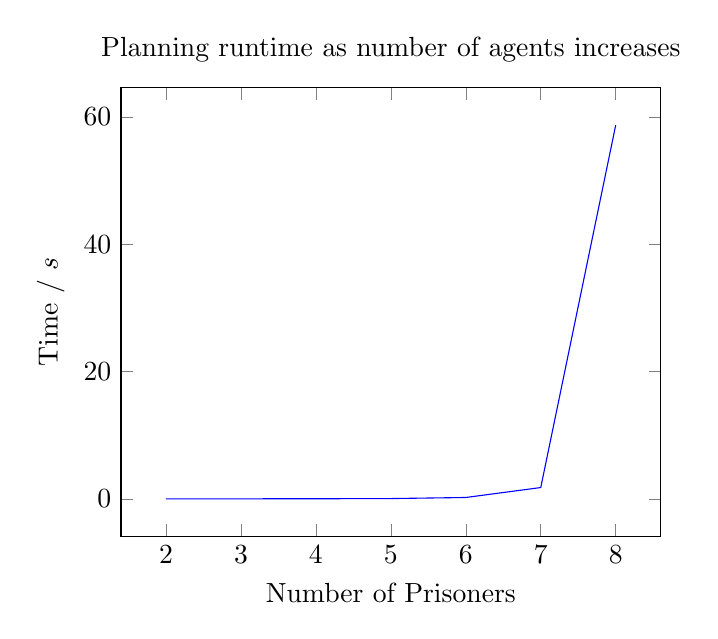
\begin{tikzpicture}
    \centering
    \begin{axis}[
      title = {Planning runtime as number of agents increases},
      xlabel = {Number of Prisoners},
      ylabel = {Time / $s$},
      ]

      \addplot[
      color = blue
      ]
      coordinates {(2, 0) (3, 0) (4, 0.01) (5, 0.04) (6, 0.21) (7, 1.77) (8, 58.71)};

    \end{axis}
  \end{tikzpicture}
  \end{subfigure}%
 ~ 
  \begin{subfigure}[b]{0.3\textwidth}
    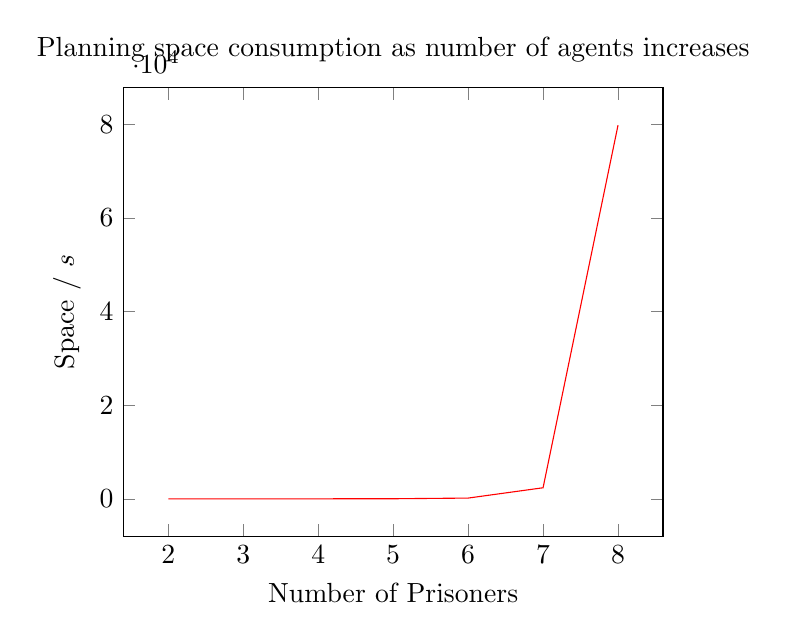
\begin{tikzpicture}
      \centering
    \begin{axis}[
      title = {Planning space consumption as number of agents increases},
      xlabel = {Number of Prisoners},
      ylabel = {Space / $s$},
      ]

      \addplot[
      color = red
      ]
      coordinates {(2, 0.11) (3, 0.459) (4, 2.78) (5, 18.478) (6, 160.479) (7, 2365) (8, 79812)};

    \end{axis}
  \end{tikzpicture}
  \end{subfigure}
  \label{fig:graphs}
  \caption{Complexity analysis graphs.}
\end{figure}

\section{Results Analysis}

\subsection{\mih{Models}}

\begin{wrapfigure}{r}{0.5\textwidth}
  \begin{center}
    \begin{minted}{haskell}
      models :: Prop p => Set.Set p -> Form p -> Bool
      models _  Top         = True
      models ps (Not form)  = not $ models ps form
      models ps (P form)    = Set.member form ps
      models ps (Or forms)  = any (models ps) forms
      models ps (And forms) = all (models ps) forms
    \end{minted}
  \end{center}
  \caption{The \mih{models} function}
  \label{fig:modelsfunction}
\end{wrapfigure}

Through looking at the cost centres given to us by GHC, we can see where our
program spends the bulk of the time computing. In our tool, the culprit is
\mih{models}, which can be seen in \figref{fig:modelsfunction}. Unfortunately
there's no more we can do to speed up this function \footnote{Short of using a
  HashSet, which gives us quicker lookup times.}, suggesting that the problem
lies in the amount of times we call it. The function is one of the essential
parts of the program; it lets us move from state to state.

The issue seems to arise from the final part of the definition of transitions in
\mestar. Recall that this is defined as:

\begin{equation} \label{eq:delta1}
  \delta(q_v, e) = q_{v'}, \text{where } v' = \{p \in \Lambda \mid v \models \post(e, p)\}
  \text{ if } 
  \models \pre(e)
\end{equation}

\noindent where, given a world where a set of propositions $v$ is true and an
event $e$, we go through each proposition $p$ in the set of propositions for the
current model and check if the set of propositions $v$ \emph{model} the postcondition
of the given proposition $p$ and the event $e$. This occurs every time we wish
to make a transition between two sets in our automata; clearly, this piece of
code is being called a lot. However, this does not seem to be a particularly bad
thing in itself; rather the opposite, it seems essential that this piece of code
would be called a lot.

\subsection{Search Strategies}

To understand the differences in efficiency, we mainly need to consider the
algorithmic differences. The other tool first enumerates the possible set of
call sequences in a depth-first manner, after which it finds the first
successful sequence of these calls. It does this latter task like a conventional
model checker, and as such can use more powerful model checking techniques. In
contrast, our tool performs a slightly different task; it builds a structure
with which it can find paths through the gossip graph, and then finds the
shortest.

The point at which this difference is really shown is in the generation of
indistinguishable states. In our tool we progressively keep track of the states
indistinguishable from our current one, and update each of these states with
each transition, leading to a lot of time spent in the \mih{models} function.
In contrast, the other tool takes the string of calls to be checked against and
generates all of the other strings of calls indistinguishable to it, and then
checks if these model the target formula. The latter technique is much more
computationally efficient than ours; the generation of these indistinguishable
call sequences is much more straightforward and requires much less heavy lifting
than maintaining this set of indistinguishable states.

% However, the method of computing these other call sequences is one that can only
% be effectively utilised when we know the 

One might ask why we don't copy this method of simply maintaining the set of
strings of indistinguishable events which could have happened in the states of
our automaton. This is a fine idea, however a problem arises when we come to
considering the successful states. In the other tool it is known that the
sequence of calls is ``final'', in the sense of a model checker - we want to
know if this is successful or it isn't. But in ours we only stop either when we
can make no more calls, or we are in a successful state. As such, we need to
know if we are in a successful state \emph{every time we enter one}, and the
only way we can do this is by performing each string of indistinguishable calls
on the initial state and evaluating the target formula at the resultant states;
it is clear that this will be less efficient.

\subsection{\mih{BFSM}}

Another method we spend a lot of time on is the BFSM method \mih{enqueue}. In
this we take the existing queue and append onto it the set of states that are
next to be visited. This function uses a lot of memory and time as it has two
memory-costly functions inside it; namely \mih{filter} and \mih{(++)}.
This was an interesting function to investigate and try and optimise. We only
need to perform two actions on our queue:

\begin{enumerate}
\item Read an item from the front
\item Append items onto the back
\end{enumerate}

In Haskell, list concatenation has runtime $O(n)$, where $n$ is the length of
the list being appended to\footnote{I.e., in the command \mih{xs ++ ys}, $n$
  is the length of \mih{xs}.}. This is far from ideal - however the
\mih{Data.Seq} package offers us constant-time access to the first and last
element of a sequence. This seems like it would be perfect for our situation,
however \textbf{for some reason currently beyond me} the time nearly doubles and
the space used balloons.

\subsection{Monotonicity}
\label{sec:Monotonicity}

Another thing we could have used to reduce computation is the monotonicity of
the propositions true at a state. At a state in the gossip protocol, if some set
$v$ of propositions are true and we make some call $e$, then the set of
propositions at the state we move to, $v'$, is guaranteed to be a superset of
$v$. Consider what this means; there is no phone call that can be made that will
make anyone know any \emph{less}. Hence we could change Equation
\ref{eq:delta1} to

\begin{equation} \label{eq:delta2}
  \delta(q_v, e) = q_{v'}, \text{where } v' = \{p \in \Lambda \setminus v \mid v \models \post(e, p)\} \cup v
  \text{ if } 
  \models \pre(e)
\end{equation}

This is because we know that the propositions in $v$ will be true at the state
$\delta(q_v, e)$; hence we do not need to check again whether or not they will
be true. 

However I fear this would be an irresponsible change to make to our code.
Remember that we do not want our system to solely plan for the Gossip problem;
rather we want it to be capable of doing so for \emph{any} epistemic model and
propositional event model. We have an example of a model where this occurs in
\figref{fig:cointoss}; although this is quite a toy example, it does indeed show
that such cases are possible. In the interests of portability then, it would be
unwise to make such a change. 

\subsection{\textsf{ANY} and related protocols}

Early on in this thesis we mentioned that \cite{GithubGossip} is unable to plan
for gossip graphs with protocols that allow for infinite call sequences (an
example of this is \textsf{ANY}). One benefit that our tool demonstrates over
\cite{GithubGossip} is the ability to plan using such protocols. This is because
before the process of searching through the gossip graph we crop the automata to
remove any calls that do not have an effect. This prevents the problem that can
arise when using \textsf{ANY}, where two agents can just repeatedly call each
other over and over again. 

This manifests itself as a great advantage over the existing tool. \textsf{ANY}
is a very practical protocol for use in the gossip problem as it requires no
reasoning on behalf of the agents; they do not need to consider whether or not
they can make a call. \textbf{Check this this is quite bad}.

\newpage

\chapter{Conclusion}

We now take some time to reflect on the work done in this project. Our
overarching aim in the project was to design an implement a system with which we
can perform epistemic planning. This document's ordering reflects the order in
which the challenges of the project were accomplished; we first reviewed the
literature, then designed the algorithm, and then implemented it. Chapters 2, 3
and 4 are respectively dedicated to each subtask.

In Chapter 2, we explained the concepts necessary to understand the algorithm
put forward. When starting work on this project the understanding of the
processes put forward in the literature was the first major difficulty, and as
such care has been taken in the writing process to make these definitions as clear
as possible. 

In Chapter 3, we put forward the algorithm designed to perform the task of
planning. We hope that this communicates the magnitude of the wrok done here, as
well as serves as a sufficient explanation for the process implemented. Whilst
the existence of this algorithm was postulated in \cite{AutomataTechniques}, it
did not exist in a simple, digestable form; the work in Chapter 3 is the first
explanation of the process in this manner. We hope that if someone were to
continue work in this area, this document would aid there understanding. 

Chapter 4 contains writing on implementation of the process. This details the
design decisions made in the process, and argues a case for the use of Haskell
in development of such a tool. 

In Chapter 5 we gave an analysis - both quantitative and qualitative - of the
work done in the thesis. 

\section{Future Work}

It is clear to see that our system is very slow; when run on a gossip graph with
greater than 6 agents the takes so long that it's not worth waiting for the
results. Whilst there is scope for implementation-based
optimisations\footnote{By which we mean optimisations like changing a
  \mih{Set} to a \mih{HashSet} and so on.}, this is mainly due to the
algorithm; in \cite{AutomataTechniques} it is shown that the propositional
epistemic planning problem is in \textsf{$k + 1$-EXPTIME}, where $k$ is the
depth of the deepest-nested knowledge operator. 

The method that we use is very explicit; we will always explore a branch, no
matter what its state is. We may be wasting computation by either exploring a
branch that is never going to succeed, or is identical to another branch. It
would be interesting to see the implementation of some checker for recomputed
branches, a la dynamic programming.

\bigskip

It also seems possible that there's scope for a symbolic approach, like in
\cite{MalvinThesis}.

\bigskip

Epistemic preconditions are investigated in \cite{EpProforDyGo}. These allow for
protocols like ``$a$ may call $b$ if $a$ knows $b$'s phone number and $a$
considers it possible that $b$ knows something that $a$ does not know.''. These
protocols are clearly much more expressive than protocols like \textsf{LNS}. In
our implementation, we encode preconditions in the \tpre function in the event
models. However, recall that in this thesis we investigate the
\emph{propositional} fragment of the epistemic planning problem, in which our
\tpre conditions may only be propositional; hence such epistemic protocols are
not possible. Despite this, there is a sensation that it would be possible to
use these protocols. We could evaluate the protocols on the states in question
, as long as they are of the \mih{PState} form. However, there might need to be
significant restructuring of the algorithm to accommodate for this; currently
protocols are restricted to just being propositional and as such are evaluated
at the atomic, \mih{PVar} states. Furthermore, it is proven in
\cite{UndecidabilityEP} that non-propositional preconditions can yield
undecidability; hence we prepare ourselves for this to not be possible. 

%%% Bibliography %%%%%%%%%%%%%%%%%%%%%%%%%%%%%%%%%%%%%%%%%%%%%%%%%%%%%%%%%%%%%%%%

\newpage

\printbibliography[title={Bibliography}]



\end{document}
